\documentclass[twoside]{article}

\usepackage{aistats2022} % aistats formatting
    % If your paper is accepted, change the options for the package
    % aistats2022 as follows:
    %
    %\usepackage[accepted]{aistats2022}
    %
    % This option will print headings for the title of your paper and
    % headings for the authors names, plus a copyright note at the end of
    % the first column of the first page.

    % If you set papersize explicitly, activate the following three lines:
    %\special{papersize = 8.5in, 11in}
    %\setlength{\pdfpageheight}{11in}
    %\setlength{\pdfpagewidth}{8.5in}

	\usepackage[american]{babel}
	\usepackage{csquotes}
	\usepackage[backend=biber, style=authoryear]{biblatex}
	\DeclareLanguageMapping{american}{american-apa}
	% \usepackage[backend=biber,style=authoryear,hyperref=true]{biblatex}
	\addbibresource{refs.bib}
	% \listfiles
	
	\DeclareFieldFormat{citehyperref}{%
	  \DeclareFieldAlias{bibhyperref}{noformat}% Avoid nested links
	  \bibhyperref{#1}}

	\DeclareFieldFormat{textcitehyperref}{%
	  \DeclareFieldAlias{bibhyperref}{noformat}% Avoid nested links
	  \bibhyperref{%
	    #1%
	    \ifbool{cbx:parens}
	      {\bibcloseparen\global\boolfalse{cbx:parens}}
	      {}}}

	\savebibmacro{cite}
	\savebibmacro{textcite}

	\renewbibmacro*{cite}{%
	  \printtext[citehyperref]{%
	    \restorebibmacro{cite}%
	    \usebibmacro{cite}}}

	\renewbibmacro*{textcite}{%
	  \ifboolexpr{
	    ( not test {\iffieldundef{prenote}} and
	      test {\ifnumequal{\value{citecount}}{1}} )
	    or
	    ( not test {\iffieldundef{postnote}} and
	      test {\ifnumequal{\value{citecount}}{\value{citetotal}}} )
	  }
	    {\DeclareFieldAlias{textcitehyperref}{noformat}}
	    {}%
	  \printtext[textcitehyperref]{%
	    \restorebibmacro{textcite}%
	    \usebibmacro{textcite}}}

	% \renewbibmacro*{cite}{%
	% 	\printtext[bibhyperref]{%
	%     \iffieldundef{shorthand}
	%       {\ifthenelse{\ifnameundef{labelname}\OR\iffieldundef{labelyear}}
	%          {\usebibmacro{cite:label}%
	%           \setunit{\printdelim{nonameyeardelim}}}
	%          {\printnames{labelname}%
	%           \setunit{\printdelim{nameyeardelim}}}%
	%        \usebibmacro{cite:labeldate+extradate}}
	%       {\usebibmacro{cite:shorthand}}}}
	% 
	% \renewbibmacro*{citeyear}{%
	%   \printtext[bibhyperref]{%
	%     \iffieldundef{shorthand}
	%       {\iffieldundef{labelyear}
	%          {\usebibmacro{cite:label}}
	%          {\usebibmacro{cite:labeldate+extradate}}}
	%       {\usebibmacro{cite:shorthand}}}}
	% 
	% \renewbibmacro*{textcite}{%
	%   \ifnameundef{labelname}
	%     {\iffieldundef{shorthand}
	%        {\printtext[bibhyperref]{%
	%           \usebibmacro{cite:label}}%
	%         \setunit{%
	%           \global\booltrue{cbx:parens}%
	%           \printdelim{nonameyeardelim}\bibopenparen}%
	%         \ifnumequal{\value{citecount}}{1}
	%           {\usebibmacro{prenote}}
	%           {}%
	%         \printtext[bibhyperref]{\usebibmacro{cite:labeldate+extradate}}}
	%        {\printtext[bibhyperref]{\usebibmacro{cite:shorthand}}}}
	%     {\printtext[bibhyperref]{\printnames{labelname}}%
	%      \setunit{%
	%        \global\booltrue{cbx:parens}%
	%        \printdelim{nameyeardelim}\bibopenparen}%
	%      \ifnumequal{\value{citecount}}{1}
	%        {\usebibmacro{prenote}}
	%        {}%
	%      \usebibmacro{citeyear}}}
	% 
	% \renewbibmacro*{cite:shorthand}{%
	%   \printfield{shorthand}}
	% 
	% \renewbibmacro*{cite:label}{%
	%   \iffieldundef{label}
	%     {\printfield[citetitle]{labeltitle}}
	%     {\printfield{label}}}
	% 
	% \renewbibmacro*{cite:labeldate+extradate}{%
	%   \printlabeldateextra}
	% \DeclareCiteCommand{\parencite}
	%   {\usebibmacro{prenote}}
	%   {\usebibmacro{citeindex}%
	%    \printtext[bibhyperref]{(\usebibmacro{cite})}}
	%   {\multicitedelim}
	%   {\usebibmacro{postnote}}
	\DeclareCiteCommand{\brakcite}
	  {\usebibmacro{prenote}}
	  {\usebibmacro{citeindex}%
	   \printtext[bibhyperref]{[\usebibmacro{cite}]}}
	  {\multicitedelim}
	  {\usebibmacro{postnote}}
	    
	% If you use natbib package, activate the following three lines:
    % \usepackage[round]{natbib}
    % \renewcommand{\bibname}{References}
    % \renewcommand{\bibsection}{\subsubsection*{\bibname}}

    % If you use BibTeX in apalike style, activate the following line:
    % \bibliographystyle{apalike}


\usepackage{tikz}
	\usetikzlibrary{positioning,fit,calc, decorations, arrows, shapes, shapes.geometric}
	\usetikzlibrary{cd}

	%%%%%%%%%%%%
	\tikzset{AmpRep/.style={ampersand replacement=\&}}
	\tikzset{center base/.style={baseline={([yshift=-.8ex]current bounding box.center)}}}
	\tikzset{paperfig/.style={center base,scale=0.9, every node/.style={transform shape}}}

	% Node Stylings
	\tikzset{dpadded/.style={rounded corners=2, inner sep=0.7em, draw, outer sep=0.3em, fill={black!50}, fill opacity=0.08, text opacity=1}}
	\tikzset{dpad0/.style={outer sep=0.05em, inner sep=0.3em, draw=gray!75, rounded corners=4, fill=black!08, fill opacity=1, align=center}}
	\tikzset{dpad/.style args={#1}{every matrix/.append style={nodes={dpadded, #1}}}}
	\tikzset{light pad/.style={outer sep=0.2em, inner sep=0.5em, draw=gray!50}}

	\tikzset{arr/.style={draw, ->, thick, shorten <=3pt, shorten >=3pt}}
	\tikzset{arr0/.style={draw, ->, thick, shorten <=0pt, shorten >=0pt}}
	\tikzset{arr1/.style={draw, ->, thick, shorten <=1pt, shorten >=1pt}}
	\tikzset{arr2/.style={draw, ->, thick, shorten <=2pt, shorten >=2pt}}

	\newcommand\cmergearr[5][]{
		\draw[arr, #1, -] (#2) -- (#5) -- (#3);
		\draw[arr, #1, shorten <=0] (#5) -- (#4);
		}
	\newcommand\mergearr[4][]{
		\coordinate (center-#2#3#4) at (barycentric cs:#2=1,#3=1,#4=1.2);
		\cmergearr[#1]{#2}{#3}{#4}{center-#2#3#4}
		}
	\newcommand\cunmergearr[5][]{
		\draw[arr, #1, -, shorten >=0] (#2) -- (#5);
		\draw[arr, #1, shorten <=0] (#5) -- (#3);
		\draw[arr, #1, shorten <=0] (#5) -- (#4);
		}
	\newcommand\unmergearr[4][]{
		\coordinate (center-#2#3#4) at (barycentric cs:#2=1.2,#3=1,#4=1);
		\cunmergearr[#1]{#2}{#3}{#4}{center-#2#3#4}
		}

\relax % Most packages
    % \usepackage[utf8]{inputenc}
    \usepackage{mathtools}
    \usepackage{amssymb}
    % \usepackage{parskip}
    % \usepackage{algorithm}
    \usepackage{bbm}
	\usepackage{lmodern}
	% \usepackage{times}
    \usepackage{faktor}
    % \usepackage{booktabs}
	% \usepackage[margin=1in]{geometry}
    \usepackage{graphicx}
    \usepackage{scalerel}
    \usepackage{enumitem}
    \usepackage{nicefrac}\let\nf\nicefrac

    \usepackage{color}
    %\usepackage{stmaryrd}
    \usepackage{hyperref} % Load before theorems...
        \hypersetup{colorlinks=true, linkcolor=blue!75!black, urlcolor=magenta, citecolor=green!50!black}

\usepackage{amsthm,thmtools} % Theorem Packages
	\usepackage[noabbrev,nameinlink,capitalize]{cleveref}
    \theoremstyle{plain}
    \newtheorem{theorem}{Theorem}
	\newtheorem{coro}{Corollary}[theorem]
    \newtheorem{prop}[theorem]{Proposition}
    \newtheorem{claim}{Claim}
    \newtheorem{remark}{Remark}
    \newtheorem{lemma}[theorem]{Lemma}
    \theoremstyle{definition}
    % \newtheorem{defn}{Definition}
    % \declaretheorem[name=Definition]{defn}
    \declaretheorem[name=Definition, qed=$\square$]{defn}

	\crefname{defn}{Definition}{Definitions}
	\crefname{prop}{Proposition}{Propositions}


\relax %%%%%%%%% GENERAL MACROS %%%%%%%%
    \let\Horig\H
	\let\H\relax
	\DeclareMathOperator{\H}{\mathrm{H}} % Entropy
	\DeclareMathOperator{\I}{\mathrm{I}} % Information
	\DeclareMathOperator*{\Ex}{\mathbb{E}} % Expectation

    \newcommand{\mat}[1]{\mathbf{#1}}
    \DeclarePairedDelimiterX{\infdivx}[2]{(}{)}{%
		#1\;\delimsize\|\;#2%
	}
	\newcommand{\thickD}{I\mkern-8muD}
	\newcommand{\kldiv}{\thickD\infdivx}
	\newcommand{\tto}{\rightarrow\mathrel{\mspace{-15mu}}\rightarrow}

	\newcommand{\datadist}[1]{\Pr\nolimits_{#1}}
	% \newcommand{\datadist}[1]{p_\text{data}}

	\makeatletter
	\newcommand{\subalign}[1]{%
	  \vcenter{%
	    \Let@ \restore@math@cr \default@tag
	    \baselineskip\fontdimen10 \scriptfont\tw@
	    \advance\baselineskip\fontdimen12 \scriptfont\tw@
	    \lineskip\thr@@\fontdimen8 \scriptfont\thr@@
	    \lineskiplimit\lineskip
	    \ialign{\hfil$\m@th\scriptstyle##$&$\m@th\scriptstyle{}##$\hfil\crcr
	      #1\crcr
	    }%
	  }%
	}
	\makeatother
	\newcommand\numberthis{\addtocounter{equation}{1}\tag{\theequation}}

\relax %%%%%%%%%   PDG  MACROS   %%%%%%%%
	\newcommand{\ssub}[1]{_{\!_{#1}\!}}
	% \newcommand{\bp}[1][L]{\mat{p}_{\!_{#1}\!}}
	% \newcommand{\bP}[1][L]{\mat{P}_{\!_{#1}\!}}
	\newcommand{\bp}[1][L]{\mat{p}\ssub{#1}}
	\newcommand{\bP}[1][L]{\mat{P}\ssub{#1}}
	\newcommand{\V}{\mathcal V}
	\newcommand{\N}{\mathcal N}
	\newcommand{\Ed}{\mathcal E}

	\DeclareMathAlphabet{\mathdcal}{U}{dutchcal}{m}{n}
	\DeclareMathAlphabet{\mathbdcal}{U}{dutchcal}{b}{n}
	\newcommand{\dg}[1]{\mathbdcal{#1}}
	\newcommand{\PDGof}[1]{{\dg M}_{#1}}
	\newcommand{\UPDGof}[1]{{\dg N}_{#1}}
	\newcommand\VFE{\mathit{V\mkern-4mu F\mkern-4.5mu E}}

	\newcommand\Inc{\mathit{Inc}}
	\newcommand{\IDef}[1]{\mathit{IDef}_{\!#1}}
	\newcommand{\ed}[3]{%
		\mathchoice%
		{#2\overset{\smash{\mskip-5mu\raisebox{-3pt}{${#1}$}}}{\xrightarrow{\hphantom{\scriptstyle {#1}}}} #3} %display style
		{#2\overset{\smash{\mskip-5mu\raisebox{-3pt}{$\scriptstyle {#1}$}}}{\xrightarrow{\hphantom{\scriptstyle {#1}}}} #3}% text style
		{#2\overset{\smash{\mskip-5mu\raisebox{-3pt}{$\scriptscriptstyle {#1}$}}}{\xrightarrow{\hphantom{\scriptscriptstyle {#1}}}} #3} %script style
		{#2\overset{\smash{\mskip-5mu\raisebox{-3pt}{$\scriptscriptstyle {#1}$}}}{\xrightarrow{\hphantom{\scriptscriptstyle {#1}}}} #3}} %scriptscriptstyle

    \newcommand{\nhphantom}[2]{\sbox0{\kern-2%
		\nulldelimiterspace$\left.\delimsize#1\vphantom{#2}\right.$}\hspace{-.97\wd0}}
		% \nulldelimiterspace$\left.\delimsize#1%
		% \vrule depth\dp#2 height \ht#2 width0pt\right.$}\hspace{-.97\wd0}}
	\makeatletter
	\newsavebox{\abcmycontentbox}
	\newcommand\DeclareDoubleDelim[5]{
	    \DeclarePairedDelimiterXPP{#1}[1]%
			{% box must be saved in this pre code
				\sbox{\abcmycontentbox}{\ensuremath{##1}}%
			}{#2}{#5}{}%
		    %%% Correct spacing, but doesn't work with externalize.
			% {\nhphantom{#3}{##1}\hspace{1.2pt}\delimsize#3\mathopen{}##1\mathclose{}\delimsize#4\hspace{1.2pt}\nhphantom{#4}{##1}}
			%%% Fast, but wrong spacing.
			% {\nhphantom{#3}{~}\hspace{1.2pt}\delimsize#3\mathopen{}##1\mathclose{}\delimsize#4\hspace{1.2pt}\nhphantom{#4}{~}}
			%%% with savebox.
		    {%
				\nhphantom{#3}{\usebox\abcmycontentbox}%
				\hspace{1.2pt} \delimsize#3%
				\mathopen{}\usebox{\abcmycontentbox}\mathclose{}%
				\delimsize#4\hspace{1.2pt}%
				\nhphantom{#4}{\usebox\abcmycontentbox}%
			}%
	}
	\makeatother
	\DeclareDoubleDelim
		\SD\{\{\}\}
	\DeclareDoubleDelim
		\bbr[[]]
	% \DeclareDoubleDelim
	% 	\aar\langle\langle\rangle\rangle
	\makeatletter
	\newsavebox{\aar@content}
	\newcommand\aar{\@ifstar\aar@one@star\aar@plain}
	\newcommand\aar@one@star{\@ifstar\aar@resize{\aar@plain*}}
	\newcommand\aar@resize[1]{\sbox{\aar@content}{#1}\scaleleftright[3.8ex]
		{\Biggl\langle\!\!\!\!\Biggl\langle}{\usebox{\aar@content}}
		{\Biggr\rangle\!\!\!\!\Biggr\rangle}}
	\DeclareDoubleDelim
		\aar@plain\langle\langle\rangle\rangle
	\makeatother


	% \DeclarePairedDelimiterX{\aar}[1]{\langle}{\rangle}
	% 	{\nhphantom{\langle}{#1}\hspace{1.2pt}\delimsize\langle\mathopen{}#1\mathclose{}\delimsize\rangle\hspace{1.2pt}\nhphantom{\rangle}{#1}}

\relax %%%%% restatables and links
	% \usepackage{xstring} % for expandarg
	\usepackage{xpatch}
	\makeatletter
	\xpatchcmd{\thmt@restatable}% Edit \thmt@restatable
	   {\csname #2\@xa\endcsname\ifx\@nx#1\@nx\else[{#1}]\fi}% Replace this code
	   % {\ifthmt@thisistheone\csname #2\@xa\endcsname\typeout{oiii[#1;#2\@xa;#3;\csname thmt@stored@#3\endcsname]}\ifx\@nx#1\@nx\else[#1]\fi\else\csname #2\@xa\endcsname\fi}% with this code
	   {\ifthmt@thisistheone\csname #2\@xa\endcsname\ifx\@nx#1\@nx\else[{#1}]\fi
	   \else\fi}
	   {}{\typeout{FIRST PATCH TO THM RESTATE FAILED}} % execute on success/failure
	\xpatchcmd{\thmt@restatable}% A second edit to \thmt@restatable
	   {\csname end#2\endcsname}
	   {\ifthmt@thisistheone\csname end#2\endcsname\else\fi}
	   {}{\typeout{FAILED SECOND THMT RESTATE PATCH}}

	% \def\onlyaftercolon#1:#2{#2}
	\newcommand{\recall}[1]{\medskip\par\noindent{\bf \Cref{thmt@@#1}.} \begingroup\em \noindent
	   \expandafter\csname#1\endcsname* \endgroup\par\smallskip}
   \setlength\marginparwidth{1.55cm}
	\newenvironment{linked}[3][]{%
		\def\linkedproof{#3}%
		\def\linkedtype{#2}%
		% \reversemarginpar
		% \marginpar{%
		% \vspace{1.1em}
		% % \hspace{2em}
		% 	% \raggedleft
		% 	\raggedright
		% 	\hyperref[proof:\linkedproof]{%
		% 	\color{blue!50!white}
		% 	\scaleleftright{$\Big[$}{\,{\small\raggedleft\tt\begin{tabular}{@{}c@{}} proof of \\\linkedtype~\ref*{\linkedtype:\linkedproof}\end{tabular}}\,}{$\Big]$}}
		% 	}%
        % \restatable[#1]{#2}{#2:#3}\label{#2:#3}%
		\marginpar{%
			% \vspace{-3em}%
			\vspace{1.5em}
			% \raggedright
			\centering%
			\hyperref[proof:\linkedproof]{%
            % \hyperref[proof:#3]{
			\color{blue!30!white}%
			\scaleleftright{$\Big[$}{\,\mbox{\footnotesize\centering\tt\begin{tabular}{@{}c@{}}
				% proof of \\\,\linkedtype~\ref*{\linkedtype:\linkedproof}
				link to\\[-0.15em]
				proof
			\end{tabular}}\,}{$\Big]$}}~
			}%
        \restatable[#1]{#2}{#2:#3}\label{#2:#3}%
        }%
		{\endrestatable%
		% \par%\vspace{-0.5em}
		% \normalmarginpar
		}
	\makeatother
		\newcounter{proofcntr}
		\newenvironment{lproof}{\begin{proof}\refstepcounter{proofcntr}}{\end{proof}}

		\usepackage[framemethod=TikZ]{mdframed}
		% \surroundwithmdframed[ % lproof
		% 	   topline=false,
		% 	   linewidth=3pt,
		% 	   linecolor=gray!20!white,
		% 	   rightline=false,
		% 	   bottomline=false,
		% 	   leftmargin=0pt,
		% 	   % innerleftmargin=5pt,
		% 	   skipabove=\medskipamount,
		% 	   skipbelow=\medskipamount
		% 	]{lproof}
	%oli16: The extra space was because there was extra space in the paragraph, not
	%because this length was too big. By breaking arrays, everything will be better.
	\newcommand{\begthm}[3][]{\begin{#2}[{name=#1},restate=#3,label=#3]}

\relax %TODOs and footnotes
    \newcommand{\TODO}[1][INCOMPLETE]{{\centering\Large\color{red}$\langle$~\texttt{#1}~$\rangle$\par}}
    \newcommand{\dfootnote}[1]{%
        \let\oldthefootnote=\thefootnote%
        \addtocounter{footnote}{-1}%
        \renewcommand{\thefootnote}{\textdagger}%
        \footnote{#1}%
        \let\thefootnote=\oldthefootnote%
    }

\begin{document}

% If your paper is accepted and the title of your paper is very long,
% the style will print as headings an error message. Use the following
% command to supply a shorter title of your paper so that it can be
% used as headings.
%
%\runningtitle{I use this title instead because the last one was very long}

% If your paper is accepted and the number of authors is large, the
% style will print as headings an error message. Use the following
% command to supply a shorter version of the authors names so that
% they can be used as headings (for example, use only the surnames)
%
%\runningauthor{Surname 1, Surname 2, Surname 3, ...., Surname n}

\twocolumn[
%%  Title objectives (might not be simultaneously satisfiable)
%%    -focus on inconsistency.  -Naturality. -Not over-reaching.
%%
% \aistatstitle{(PDG) Inconsistency: the Universal Loss}
% \aistatstitle{Choose your Model, not your Loss:}
% \aistatstitle{Loss Functions are the Shadows of Inconsistent Models}
% \aistatstitle{Loss Functions are the Shadows of Inconsistent Models (Choose your Model, not your Loss)}
% \aistatstitle{Loss Functions are the Shadows of Inconsistent Models}
% \aistatstitle{Inconsistency, the Universal Loss Fuction: How Loss is but the Shadow of an Inconsistent Model}
% \aistatstitle{Inconsistency, the Universal Loss Fuction: Our Favorite Objectives are but  Shadows of Inconsistent Models}
% \aistatstitle{The One True Loss: How Our Objectives are but Shadows of Inconsistent Models}
%
% \aistatstitle{Probabilistic Dependency Graphs: Model Inconsistency as the Universal Loss Function}
% \aistatstitle{Inconsistency, the Universal Loss Fuction: Our Favorite Objectives are mere shadows of Probabilistic Dependency Graphs}
% \aistatstitle{Choose your Model, not your Loss Function: Objectives are the Shadows cast by Inconsistent Probabilistic Dependency Graphs}
% \aistatstitle{Loss Functions are mere Shadows of Probabilistic Dependency Graphs: Choose your Model, not your Loss}
% \aistatstitle{Inconsistency from Probabilistic Dependency Graphs: Choose your Model not Your Loss.}
% \aistatstitle{ The Shadows of an Inconsistent Probabilistic Dependency Graphs: \\
	% Choose your Model, not your Loss Function}
\aistatstitle{ Inconsistency of : \\
	Choose your Model, not your Loss Function}


\aistatsauthor{ Oliver E. Richardson }
\aistatsaddress{ Cornell University } ]

\begin{abstract}
    % The Abstract paragraph should be indented 0.25 inch (1.5 picas) on
    % both left and right-hand margins. Use 10~point type, with a vertical
    % spacing of 11~points. The \textbf{Abstract} heading must be centered,
    % bold, and in point size 12. Two line spaces precede the
    % Abstract. The Abstract must be limited to one paragraph.
    % I will argue that minimizing PDG inconsistency is actually much more broadly useful, and in particular show that many standard loss functions arise as the inconsistency of the natural PDG describing the appropriate scenario.  We will then see how the extra structure of the underlying PDGs gives a rich visual proof language for reasoning about the relationships between objectives.
    In a world blessed with a great diversity of loss functions, 
    we argue that that choice between them is not a matter of taste, but a modeling assumption.
	Probabilistic Depencency Graphs (PDGs) are probabilistic models
    that can capture inconsistency.
	%joe1: This is the first of many places where you assume the reader
	%knows what you know, although that's unlikely to be true.    The
	%reader won't know that we can talk about the inconsistency of a PDG.
	    %Added next sentence
	We can associate with each PDG its \emph{inconsistency}, a measure of
	the degree to which the PDG is inconsistent.
    We prove that many standard objectives are the incinstencies of
	%joe1: I doubt it's unique in general
	%    the natural PDG describing the scenario at hand, and corroborate
    a natural PDG describing the scenario at hand.
	%joe1: this is out of place, and mysterious
	%    and corroborate an existing connection between regularizaters and
	%    priors.  
	    % We then focus on two surprising examples.
	%joe1
	    %    We then show that PDGs generate a large class of statistical
        We then show that the incnosistency of PDGs can capture a
	        large class of statistical 
	    divergences, and detail the benefits of doing so, including a
	    visual proof language for proving inequalities between them. 
	    Finally, we focus turn to variational inference, and show that the
	%joe1
	%    ELBO, a difficult-to-motivate function for training Variational
	    ELBO, a difficult-to-motivate function for training variational
	    models, and its variants arise for free out of the modeling assumptions, as 
	%joe1: singular or plural
	% do an intuitive visual proofs of the variational bounds used to motivate
	 does an intuitive visual proof of the variational bounds used to motivate
	 it.
	%joe1: idf you feel a great need to talk about regularizer, say
	%something like  s(It seems strange to say "In addition" after
	%"Finally"; you may want to smooth the wording if you add this.
	In addition, we show that PDGs can be used to justify a well-known
	connection between regularizers and priors.
\end{abstract}

\section{INTRODUCTION}
% \section{CHOOSE YOUR MODEL, NOT YOUR LOSS}
% -universality
Many tasks in artificial intelligence have been fruitfully cast as optimization problems, but often the choice of objective is not unique.
%
% For instance, one key component of a machine learning system is a
% `loss' that the system tries to minimize, and many different
% formulas (such as hinge loss, cross entropy, mean squared error, and
% accuracy) are commonly employed. 
For instance, a key component of a machine learning system is a loss
%joe1: must minimize?  This is the first of many run-on sentences
%function which the system to minimize, and a wide variety of such
function which the system must minimize.  A wide variety of such
functions are used in pratice.
%oli2: removed examples
% (e.g., cross entropy, square error, hinge loss, \ldots). 
% In machine learning, the objective is often called the loss function, and many different
%oli: this sentence perhaps unnecessary...
% All are backed by a similar intuitions of `proximity to ground truth', but draw from different formalisms.
Each implicitly represents different values, and results in different
%joe1: another run on
%behavior, and so the choice of loss can be quite important---and yet
behavior, so the choice of loss can be quite important
%TODO VET THIS
% \parencite{wang2020comprehensive}
% \parencite{jadon2020survey}.   
\parencite{wang2020comprehensive,jadon2020survey}
Yet,
%joe1*: do you have examples or references you can cite?   This is
%strong claim, and needs some defence.  
because the crieteria for choosing a ``good'' loss function are often
inscrutible, the choice is usually made by instinct, tradition, or to
simplify implementation, rather than because it reflects one's beliefs.
%joe1: Ddon't bring in values.  These involve utilities, and you never
%mention utilities in the paper 
%or values.  
%We aim to
Furthermore, there is something to be gained by fiddling with these
loss functions: one can add regularization terms, to (dis)incentivize
(un)desirable behavior.
%joe1: again, a reference where this is done would be useful here
%But this process---of tinkering with the objective and afterwards
%TODO
But this process---tinkering with the objective and afterwards
spinning a story about why it works---is unsatisfying.
%joe1: another run-on
%it can be a tedious game without clear rules or meaning, and results
%oli1: I want these two thoughts to be connected. 
% it can be a tedious game without clear rules or meaning. Results so obtained are arguably overfitted and pedagogically difficult to motivate. 
It can be a tedious game without clear rules or meaning,
 % while results so obtained are arguably overfit and difficult to motivate. 
 that brings 
%
% We attribute this state of affairs to the relative permisiveness of the medium of expression.
% ...


By contrast, a choice of \emph{model} admits more principled
discussion, in part because it makes sense to ask if a model is
accurate, or of it captures a real phenomenon.
%joe1: this is out of place. The reader will have no idea what "model
%inconsistency" is, let alone know that we're interested in a measure
%of it.   It also breaks the flow.  
%This observation motivates our proposal: the use of model
%inconsistency a ``universal'' loss function.
In this framework, it is
no longer possible to specify an objective directly; rather, one must
articulate a situation that gives rise to it, in the (more
interpretable) language of probablistic beliefs and certainties. % (concretely, as a PDG \cite{richardson2020probabilistic}). 
Concretely, we use the machinery of Probabilistic Dependency Graphs
%joe1
%(PDGs), a particularly expressive class graphical models which can can
(PDGs), a particularly expressive class graphical models that can can
incorporate aribtrary (even inconsistent) probabilistic information in
a natural way, and comes equipped with a well-motivated measure of
inconsistency  \parencite{richardson2020probabilistic}. 


%joe1*: perhaps add the following sentence
The goal of this paper is to show that we can use PDGs and their
associated measure of inconsistency to proide a model-based 
``universal'' loss function.
%joe1
%In this paper, we show that many standard objective functions---cross
Towards this end, we show that many standard objective functions---cross
entropy, square error, many statistical distances, the ELBO,
regularizers, and the log partition
%joe1
%function--- arise naturally as inconsistencies of the appropriate
function---arise naturally as inconsistencies of the appropriate
underlying PDG. 
%joe1: I would tonie this down; also clarify what purpose you have in mind
%This is especially surprising because PDGs were not designed for this purpose. 
This is somewhat surprising, since PDGs were not designed with the
goal of capturing loss functions at all.
% which surprised us because it was not designed with any of them in
% mind, but rather from purely information-theoretic considerations.
%joe1: What do you mean by "schme of objective specification?  Do you
%mean using models?  What's objective about that?
%Such a scheme of objective specification may be more restrictive, but
%oli1: oops, I meant objective as the synnonym for loss. Your reword
% is ok, but verbose and not as clean as I was trying for. I'm trying again.
%% Using models (specifically, PDGs) and inconsisstency to specify an
%% objective  may be more restrictive than using loss functions,
Specifying a loss function indirectly like this may be more restrictive,
but it is also more intuitive
(since familiarity with  losses is no longer required), and admits more 
%joe1: what do you mean by "epistemically grounded"?  Do you mean
%something like "and forces the agent to express their beliefs"?  If
%so, say that.  It's much less mysterious.  The reader does not have
%access to your mind! 
%oli1: I think I mean a combination of things:
%  - 
%% grounded support and criticism. 
epistemically grounded criticism and defense.
% This change is analogous to a higher-level programming language, which restricts the set of legal programs but also makes programs easier to reason about, and ultimately,  even easier to write.


%TODO Variational AutoEncoder
% From our notion of inconsistency.
% Furthermore, this approach unifies the semantics of standard graphical models, such as BNs and factor graphs % TODO
% and illustrate by example how often

For a particularly powerful demonstration, consider the variational
%joe1: you nee4 a reference here
autoencoder (VaE), an enormously successful class of generative model
that has enabled breakthroughs in image generation, semantic
interpolation, and unsupervised feature learning. 
Structurally, a VaE for a space $X$ consists of a (smaller) latent space $Z$, a prior distribution $p(Z)$, a decoder $d(Z | X)$, and an encoder $e(Z| X)$.
% Despite the fact that they are usually introduced by way of a graphical model (the Bayesian Network
%     % $\xrightarrow{p} Z \xrightarrow{d} X$
%     comprising the prior $p(Z)$ and decoder $d(X|Z)$),
A VaE is not considered a ``graphical model'' for two reasons.
The first is that the encoder $e(Z|X)$ has the same target variable as $p(Z)$, so a standard directed graphical model cannot simultaneously incorporate them both (after all, they could be inconsistent with one another).
The second reason: it is not a VaE's structure, but rather its \emph{loss function} that makes a VaE tick. A VaE is typically trained by 
    % minimizing a function called the Evidence Lower BOund (ELBO), 
maximizing the ``ELBO'', 
    a somewhat difficult-to-motivate function of a sample $x$, borrowed from variational analysis.
%joe1:? 
%oli1: it's the negative ELBO (to maximize elbo, minimize inconsistency).
% also, I don't have space for all the references, so I won't include any of them.
%    We show (\Cref{prop:pdg-elbo-x}) that $-\mathrm{ELBO}(x)$ is also
    We show that $\mathrm{ELBO}(x)$ is also
    precisely the inconsistency of a PDG containing the probabilistic
    information of the autoencoder ($p, d$, and $e$) and the sample $x$.
%joe1: stress the goodness of PDGs!
% We can find such a PDG precisely because PDGs let us capture inconsistencies.     
%oli1: I find that sentence strange. 
%TODO: reword.
% We can form such a PDG precisely because PDGs allow for inconsistency.
% Thus, PDG semantics simultaneously legitimize the strange structure
% the VaE, and also justify its loss function, which can be thought of
% as a property of the model itself (its inconsistency), rather than
% some mysterious construction borrowed from physics. 
Thus, PDG semantics simultaneously legitimize the strange structure
the VaE, and also justify its loss function, which can be thought of
as a property of the model itself (its inconsistency), rather than
some mysterious construction borrowed from physics. 



%%%%%%%%%%%%%%%%%

Representing objectives as model inconsistencies, in addition to providing a principled way of selecting an objective, also has beneficial pedagogical side effects, because of the relationships between the underlying models.
%joe1: 
%For instance, we will be able to use the structure to give rise to
For instance, we will be able to use the structure of the PDG to give rise to
very simple and intuitive proofs of otherwise unintuitive results,
%oli1: 
% such as the variational inequalitites to which the ELBO owes its name,
% and the monotonicity of R\'enyi entropy  in its parameter $\alpha$. 
such as the variational inequalitites that traditionally motivate the ELBO,
and the monotonicity of R\'enyi divergence.

% Is there a deeper reason to use one measure of  these terms?

% % This state of affairs presents some problems. One is scientific.
% Another is pedagogical. Where does cross-entropy come from? What about the ELBO?


% In the coming sections, we will show in more detail how this concept of inconsistency, beyond simply providing a forgiving and intuitive modeling framework, reduces exactly to many standard objectives used in machine learning, measures of statistical distance, and also demonstrate that this framework clarifies the relationships between them, by providing simple clear derivations of otherwise opaque inequalities.
In the coming sections, we will show in more detail how this concept of inconsistency, beyond simply providing a permissive and intuitive modeling framework, reduces exactly to many standard objectives used in machine learning, measures of statistical distance, and also demonstrate that this framework clarifies the relationships between them, by providing simple clear derivations of otherwise opaque inequalities.
% we can capture regularizers in a way that justifies a well-known connection between priors and regularizers

%TODO
% \TODO[FOLD IN REGULARIZERS AGAIN]
% %joe1: in general, it's bad form to have a single subsection.  It also
% %seems strange to have a single paragraph subsection coming at the
% %end.  Fold it in to the rest!  Moreover, it's hard to imeagine that
% %the only work related to this is work on regularizers.
% %\subsection{Related Work}
% 
% %joe1: tried to provide glue, but I dont' think it's very good.  
% %Recent work in the Bayesian ML community has established a
% Using PDGs and their inconsistency allos allows us to provide a
% justification for recent work
% that has established a
% correspondence between regularizers and priors 
% \cite{williams1995bayesian,rennie2003l2,probinterptowardsds,probinterpblogpost}.
% A primary motivation for this line of work is the ability it gives us to view regularizers as \emph{prior beliefs}, which, because they are modeling assumptions, makes them better targets for principled discussion and criticism.
% %joe1*: what does "compatible" mean?  Also, what does this have to do
% %with all the work on lss functions that you've discussed up to now.
% %This seems like a disconnected random observation.  You need to tie
% %it in better.
% In \cref{sec:regularizers} we show how our approach is compatible with
% these results, and can be thought of as a natural extension of them. 


\section{PRELIMINARIES}
We generally use capital letters for variables, and lower case letters for their values.
% We use letters of both cases for conditional probability distributions (cpds), which we generally conflate their with probability mass functions.
For variables $X$ and $Y$, a conditional probability distribution (cpd) $p$ on $Y$ given $X$, written $p(Y|X)$, consists of a probability distribution on $Y$ (denoted $p(Y\mid X\!=\!x)$ or $p(Y\mid x)$ for short), for each possible value $x$ of $X$.
%joe1
%If $\mu$ is a probability on outcomes which determine $X$ and $Y$,
If $\mu$ is a probability on outcomes that determine $X$ and $Y$,
then $\mu(X)$ denotes the marginal of $\mu$ on $X$, and $\mu(Y|X)$
denotes the conditional marginal of $\mu$ on  $Y$ given $X$. 
% Conditional probability distributions (cpds) are  $p(Y|X)$
% For instance, a given a conditional probability measure $\Pr$ on $Y$ given $X$, with a mass function $p$, we write  $p(Y\mid X)$ for the cpd $(x,y) \mapsto p.\text{pmf}(y \mid x)$.
Depending on which we find clearer in context, we write either $\Ex_\mu f$ or $\Ex_{\omega \sim \mu} f(\omega)$ for expectation of $f : \Omega \to \mathbb R$ over a distribution $\mu$ with outcomes $\Omega$.
We write $\kldiv\mu\nu = \Ex_\mu \log \frac{\mu}{\nu}$ for the relative entropy (KL Divergence) of $\nu$ with respect to $\mu$, and for finitely supported $\mu$, we write $\H(\mu) := \Ex_\mu \log\frac1\mu$ for the entropy of $\mu$, $\H_\mu(X):= \H(\mu(X))$ for the marginal entropy on a variable $X$, and $\H_\mu(Y \mid X):= \Ex_\mu \log \nicefrac1{\mu(Y|X)}$ for the conditional entropy of $Y$ given $X$.

%joe1
%A Probabilsity Dependency Graph (PDG)
A \emph{probabilistic dependency graph} (PDG)
\parencite{richardson2020probabilistic}, like a Bayesian Network (BN), is a
directed graph with cpds attached to it. While this data is attached
to the \emph{nodes} of a BN, it is attached to the \emph{edges} of
PDG. 
% Concretely, while in a BN, the variable $X$ is associated with the distribution $\Pr_X(X \mid \mathbf{Pa}(X))$ on $X$ given its parents, an edge $\ed LXY$ of a PDG is associated with a distribution $\Pr(Y \mid X)$.
% As a result, a PDG of shape $X \to Y \leftarrow Z$ gives a cpd $p(Y\mid X)$ on $Y$ given $X$ and also (separately) a cpd $q(Y \mid Z)$ on $Y$ given $Z$, while a BN of the same shape has a single cpd $\Pr(Y \mid X,Z)$ on $Y$ given joint values of $X,Z$.
For instance, a PDG of shape $X \to Y \leftarrow Z$ contains both cpd $p(Y | X)$ and a cpd $q(Y | Z)$, while a BN of the same shape has a single cpd $\Pr(Y | X,Z)$ on $Y$ given joint values of $X,Z$.
The first interpretation is more expresive, and can encode joint dependence with an extra variable and pair of edges.
% Formally, the syntax of a PDG is given in \cref{defn:pdg}.
We now restate the formal definition.
% from \cite{richardson2020probabilistic}.

\begin{defn}
    %[Richardson \& Halpern
    \label{defn:pdg}
	A Probabilistic Dependency Graph (PDG) is a tuple $\dg M = (\N,\Ed,\V,\mat p, \boldsymbol\alpha, \boldsymbol\beta)$, where
    \vspace{-1em}
	%joe1: You seem to have worked hard on this, and I found it ugly.  I think bullets are much more helpful
	%oli1: The bullets look better than I thought.
	%\begin{description}[leftmargin=1em,labelindent=1.5em,itemsep=0pt]
    \begin{itemize}[leftmargin=1.5em, itemsep=0pt]
		% \item[$\N$]
        \item $\N$
			is a set of nodes, corresponding to variables;
		%joe1
		% \item[$\V$]
		\item $\V$
			associates each node $X \in \N$ with a set $\V(X)$ of possible values that the variable $X$ can take;
            % making it a variable;
		%joe1
		% \item[$\Ed$]
   		\item $\Ed$
			is a set of labeled  edges $\{ \ed LXY \}$, each with a source
			$X$ and target $Y$ from $\N$;
			% is a set of labeled  edges $\{ \ed L{\mat X}{\mat Y} \}$, each with a source
			% $\mat X$ and target $\mat Y$ subset of $\N$;
		%joe1
		% \item[$\mat p$]
        \item $\mat p$
		associates
        a cpd $\bp(\mskip-1muY\mskip-1mu|\mskip-1muX\mskip-2mu)$
        to each edge $\ed L{X\!\!}{\!Y} \!\in\! \Ed$;
		% associates to each edge $\ed L{\mat X}{\mat Y} \in \Ed$
		% a conditional probability $\bp(\mat Y\mid\mat X)$ on $\mat Y$ given $\mat X$;
		% --- that is,
		% a conditional distribution
        % a cpd $\bp(Y|X)$ --- that is, a distribution
        % $\bp(Y \mid x)$ over $Y$ for each $x \in \V(X)$;
		% a distribution $\bp(x)$ on $Y$ for each $x \in \V(X)$;
		%joe1
		% \item[$\boldsymbol\alpha$]
		\item $\boldsymbol\alpha$
		associates to each edge $\ed L{X}{Y}$ a non-negative number $\alpha_L$
	     % which, roughly speaking, is
	    % the modeler's confidence in the functional dependence of $Y$ on the variables $X$ implicit in $L$;
	    % which, roughly speaking, is
	    % representing% the modeler's confidence in the functional dependence of $Y$ on $X$;
	    representing
	    the modeler's confidence in the functional dependence of $Y$ on $X$;

		%joe1
		%\item[$\boldsymbol\beta$]
		\item $\boldsymbol\beta$
		associates to each edge $L$ a real number $\beta_L$,
		the modeler's subjective confidence in the reliability of
	    % indicating the agent's trust in the reliability of
		%added now that there's an extra line
		the cpd
		$\bp$.%
	    % \vspace{-2em}%
	    \qedhere
	%joe1
	% \end{description}%
    \end{itemize}%
\end{defn}

% This presentation is looks slightly different from the original presentation in \cite{richardson2020probabilistic}, but is equivalent.
This presentation is equivalent to one in which edge sources and targets are both \emph{sets} of variables.
% \cite{richardson2020probabilistic}.
This allows us to indicate joint dependence with multi-tailed arrows, joint distributions with multi-headed arrows,
and unconditional distributions with nothing at the tail. For instance, we will draw
%oli2:
$p(X)$ as \tikz[baseline=-0.1ex] \draw[arr2,<-] node[dpad0] (X){$X$} (X) -- node[above, inner sep=1pt]{$p$} ++(-1,0);\,,
\[
	% p(Y|X,Z)~
	% \text{as}~
	p(Y|X,Z)~\text{as}~
	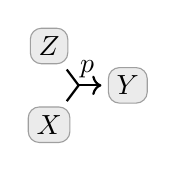
\begin{tikzpicture}[center base]
		\node[dpad0] (Y) at (1,0) {$Y$};
		\node[dpad0] (X) at (0,-0.5) {$X$};
		\node[dpad0] (Z) at (0, 0.5) {$Z$};
		\mergearr[arr2] XZY
		\node[above right=-1pt and -3pt of center-XZY] {$p$};
	\end{tikzpicture}~,
    % ~~\text{and $q(Y)$ as }~~
	% \begin{tikzpicture}[center base]
	% 	\node[dpad0] (Y) at (1,0) {$Y$};
	% 	\draw[arr2, <-] (Y) -- node[left,inner sep=2pt]{$q$} ++(0,1);
	% \end{tikzpicture}~.
    ~\text{and $q(A,B)$ as }~
	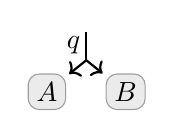
\begin{tikzpicture}[center base]
		\node[dpad0] (A) at (0,0) {$A$};
        \node[dpad0] (B) at (1,0) {$B$};
        \coordinate (above) at (0.5,0.8);
        \coordinate (center) at (0.5,0.4);
		% \draw[arr2, <-] (Y) -- node[left,inner sep=2pt]{$q$} ++(0,1);
        \cunmergearr[arr1] {above}{A}{B}{center}
        \node[above left=0pt and 0pt of center,inner sep=2pt]{$q$};
	\end{tikzpicture}\,.
 \]
% \TODO[SLOW DOWN]
%joe1*: you need to SLOW DOWN here and reimnd the reader what these
%pictures are saying.  They do not have access to your mind
%oli1: added one more example. 

% An unconditional distribution $p(X)$ can be given by associating it to a hyper-edge $\emptyset \to \{X\}$, or directly by \cref{defn:pdg} by taking its source to be a ``variable'' that can only take on one possible value.
% We will not make much use of $\alpha$ here, so $\mat p$ and $\beta$ are the most important

Like other graphical models, PDGs have semantics in terms of joint distributions $\mu$ over all variables.
% Most directly, a PDG $\dg M$ determines two scoring functions on joint distributions $\mu$, which measure the discrepency between $\dg M$ and $\mu$. The \emph{incompatibility} of $\mu$ with respect to $\dg M$, which measures the quantitative discrepency between $\mu$ and the cpds of $\dg M$, is given by
Most directly, a PDG $\dg M$ determines two scoring functions on joint
%joe1
%distributions $\mu$. For us, the more important of the two is the
distributions $\mu$. For the purposes of this paper, the more
important of the two is the 
\emph{incompatibility} of $\mu$ with respect to $\dg M$, which
measures the \emph{quantitative} discrepency between $\mu$ and the
cpds of $\dg M$, is given by 
\begin{equation}
	% \bbr{\dg M}_\gamma(\mu) = \gamma \IDef{\dg M}(\mu) +  \sum_{\ed LXY} \Ex_{x \sim \mu(X)} \beta_L \kldiv[\Big]{\mu(Y\mid x)}{\bp(Y \mid x)}
    \Inc_{\dg M}(\mu)\! := \!\!\!\sum_{\ed LXY}\!\! \beta\ssub L \!\cdot\!\!\! \Ex_{{x \sim \mu(\mskip-2.6muX\mskip-2mu)}} \kldiv[\Big]{\mu(Y|\, x)}{\bp(Y |\, x)}.
	% \label{eq:semantics}
    \label{eq:inc}
\end{equation}
% For the examples here, we can select $\alpha$ such that $\IDef{\dg M}(\mu) = 0$ for all $\mu$, and we can also set $\gamma=0$ to ignore it explicitly.
% There is more than one coherent interpretation of this expression; here is one based on codes.
It is well known that $\kldiv{\mu}{p}$ is a measure of divergence between $\mu$ and $p$, which can be interpreted as overhead (in extra bits per sample) of using codes optimized for $p$, when in fact samples are distributed according to $\mu$ \parencite{mackay2003information}.
% $\Inc_{\dg M}$ penalizes a candidate distribution $\mu$ for every deviation from a cpd $\bp[L](Y\mid X)$, in proporition to the number of bits needed to transmit samples from $\mu(Y\mid X)$ with a code optimized for the agent's belief $\bp[L](Y\mid X)$, scaled by the confidence of the edge
%joe1
%But if one uses edges in proportion to the condfidence one has in
But if one uses edges in proportion to the confidence one has in
them, then $\mu$'s violations of high-confidence cpds are compounded,
and hence more costly. 
So $\Inc_{\dg M}(\mu)$ measures the total expected excess cost of
%using the cpds of $\dg M$ in proportion to their confidences, in a
%joe1: PDGs don't hae confidences; modelers do
% using the cpds of $\dg M$ in proportion to the confidence the modeler has in them, in a
%oli1: this is more lengthy, and I think an overly pedantic distinction,
% since we've alredy said confidences are "associated to edges"
using the cpds of $\dg M$ in proportion to the confidence the modeler has in them, in a
world drawn from $\mu$. 
%
% In general, we do not know the true distribution $\mu$, only the model $\dg M$, which we interpret as charitably as possible
% (even though it might be inconsistent).
% In general, we do not know the true distribution $\mu$, only the model $\dg M$.
% So, under the assumption that
The \emph{inconsistency} of $\dg M$, denoted
$
    \aar{\dg M} := \inf_\mu \Inc_{\dg M}(\mu),
$
is the smallest possible incompatibility with any distribution
%joe1
%    is the smallest possible incompatibility with any distribution.
%oli1: reverse order.
% is the smallest possible incompatibility of the PDG $\dg M$ with any distribution. 
is the smallest possible incompatibility of any distribution with respect to $\dg M$.


The second scoring function defined by a PDG $\dg M$, called information deficiency, measures the \emph{qualitative} discrepency between $\dg M$ and $\mu$, and is given by
\[ \IDef{\dg M}(\mu) := -\H(\mu) + \sum_{\ed LXY} \alpha\ssub L \H_\mu(Y\mid X). \]
$\IDef{\dg M}(\mu)$ can be thought of as measuring the
% additional entropy in the $\mu$ beyond what one would expect from the link structure alone, and captures
(weighted) number of bits needed to describe the target of each edge given its source, beyond the information needed to describe a full sample of $\mu$.

%joe1
%It is via these two scoring functions that PDGs capture other
% As shown in \cite{richardson2020probabilistic}, 
%oli1: unfortunately the guide wants it to 
As shown by \textcite{richardson2020probabilistic},
it is via these two scoring functions that PDGs capture other
graphical models: the distribution specified by a BN $\dg B$ is the
unique one that minimizes both $\Inc_{\dg B}$ and $\IDef{\dg B}$ (and
hence every positive linear combination of the two), and the
distribution specfied by a factor graph $\Phi$ uniquely minimizes the
sum $\Inc_{\Phi} + \IDef{\Phi}$. 
In general, for any $\gamma > 0$, the one can consider a weighted combination
\(
    \bbr{\dg M}_\gamma(\mu) \!:= \Inc_{\dg M}(\mu) + \gamma\; \IDef{\dg M}(\mu),
\)
for which there is a corresponding $\gamma$-inconsistency $\aar{\dg M}_\gamma := \inf_\mu \bbr{\dg M}_\gamma(\mu)$.
% It is shown in \cite{richardson2020probabilistic} that
In the limit as $\gamma \to\! 0$, there is always a unique best distribution
%$\mu^*$
whose score is
% $\bbr{\dg M}_0(\mu^*) = \Inc_{\dg M}(\mu^*) = \aar{\dg M}_0 = \aar{\dg M}$.
$\aar{\dg M}$.

% The \emph{best} distribution by this metric (the one with the smallest loss), denoted $\bbr{\dg M}_\gamma^*$,
% = \arg\min_\mu \bbr{\dg M}(\mu)$
% exists and is unique for small enough $\gamma$, and also in the limit as $\gamma$ goes to zero;
% we write $\bbr{\dg M}^*$, without a subscript, to indicate this limiting best joint distribution.
% It is via this joint distribution that PDGs generalize other graphical models

% here we argue that the scoring function \eqref{eq:semantics} encodes useful information beyond its minimizer.

% The value of \eqref{eq:semantics} achieved by this optimal distribution is called the \emph{inconsistency} of $\dg M$, and is denoted $\aar{\dg M}_\gamma$.
% Because we can essentially set $\IDef{} = 0$ with certain neutral choices of $\alpha$, and because $\IDef{}$ is not the focus of this paper, we will often drop the subscript $\gamma$.
% Any such formula can be interpreted litterally by setting $\gamma = 0$, and our results can be extended for other values of $\gamma$ with more careful treatmeant of the qualitative half of the picture.
% In a select few places, we will point out the qualitative term.
 % := \inf_\mu \bbr{\dg M}(\mu)$.


%joe1:
%Now, some short-hand.
% We noe present some shorthand and abbreviations t hat makes the prsentation of PDGs simpler.  
%oli1:
% We noe present some shorthand and abbreviations t hat makes the prsentation of PDGs simpler.  
We now present some shorthand to simplify the presentation.  
% By default, all cpds are associated with confidence $\beta = 1$.
%joe1: do we actually ever do it?

\TODO{SORT OUT}

A cpd $p$ can be regarded as a PDG with a single edge (with $\bp[p] =
p$, and  $\alpha_p=0$ and $\beta_p = 1$ by default), and sometimes we
make this conversion implicitly.
% p$, and  $\alpha_p=0$ and $\beta_p = 1$;   we sometimes do so.
% union is not really used.
The union of $\dg M$ and $\dg M'$ is denoted by $\dg M + \dg M'$.
We identify an event $X=x$ with with the degenerate distribution on $X$ that places all mass on $x$, and hence may be associated to an edge.
%joe1
%Furthermore, as is unambiguous to shorten this event to simply $x$, as
%the label of an edge.
We occasionally write $x$ rather than $X=x$ as the label of the edge.
To emphasize that an edge is degenerate (a function), we will draw it
%joe1*: Draw an example!
with two heads.  
To specify a confidence $\beta \ne 1$, we put it in a parentheses
%joe1*: why a lighter color?  This makes it harder to read, and does
%not help (at least, not me) in any way.  I strongly recommend that
%you don't use a lighter color
and a lighter color nearby the edge, as in
% % By default, all cpds are associated with confidence $\beta = 1$.
% A cpd $p$ can be regarded as a PDG with a single edge (with $\bp[p] = p$, and  $\alpha_p=0$ and $\beta_p = 1$ by default), and sometimes we make this conversion implicitly.
% %% union is not really used.
% % The union of $\dg M$ and $\dg M'$ is denoted by $\dg M + \dg M'$.
% We identify an event $X=x$ with with the degenerate distribution on $X$ that places all mass on $x$, and hence may be associated to an edge.
% Furthermore, as is unambiguous to shorten this event to simply $x$, as the label of an edge.
% To emphasize that an edge is degenerate (a function), we will draw it with two heads. 
% To specify a confidence $\beta \ne 1$, we put it in a parentheses and a lighter color nearby the edge, as in
% $p ~^{\color{gray}{(\beta\colon0.7)}}$, or
% $p^{\color{gray}(\beta)}$ as a compressed form of
% of $p^{\color{gray}{(\beta:\beta)}}$.
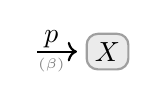
\begin{tikzpicture}[center base]
    \draw[arr, <-] node[dpad0](X){$X$} (X) --
        node[above,pos=0.6, inner sep=1pt]{$p$}
        node[below,pos=0.6, inner sep=2pt]{${\scriptscriptstyle\color{gray}(\beta)}$}
         ++(-1,0);
\end{tikzpicture}.
%
%joe1*: I think that this is a bad idea.  Help the reader and use
%\beta \to \inftyh.  You may be used to your notation, but the typical
%reader will absolutely not be.
We use ${\scriptstyle\color{gray}(\infty)}$ to denote the limit of high confidence ($\beta \to \infty$).
% To inciate the limit of high confidence on a cpd $p$, we write an exclamation point, as in: \tikz[baseline=0.9] \draw[arr, <-] node[dpad0](X){$X$} (X) -- node[below,pos=0.6, inner sep=2pt]{$p!$} ++(-1,0);.
 % ($\beta_p \to \infty$)


\subsection{Monotonicity of Inconsistency}


% It is easy to show that adding edges, or increasing their confidences, cannot decrease the inconsistency of a PDG.
Intuitively, believing more things can't make you any less inconsistent.
\Cref{lemma!}, our workhorse lemma for deriving relationships between loss functions, captures this formally: adding edges, or increasing confidences, cannot decrease the inconsistency of a PDG.

\begin{lemma}[monotonicity of inconsistency]\label{lemma!}
 	For all pdgs $\dg M$ and $\dg M'$, with respective confidence vectors $\beta$ and $\beta'$, we have that
	\begin{enumerate}[label={\arabic*.}]
		%TODO
		%joe1: the + notation is undefined
		\item  $\aar{\dg M + \dg M'}_\gamma \ge \aar{\dg M}_\gamma$.
		%oli1: another possibility
		% \item  $\aar{\dg M + \dg M'}_\gamma \ge \aar{\dg M}_\gamma$,
			%where $\dg M + \dg M'$ is the union of $\dg M$ and $\dg M'$. 
		\item If
            % and $\beta \succeq \beta'$ (that is, $\beta_L \ge \beta'_L$ for all $L \in \Ed$), then $\aar{\dg M} \ge \aar{\dg M'}$.
            $\beta_L \ge \beta'_L$ for all $L \in \Ed$, then $\aar{\dg M} \ge \aar{\dg M'}$.
	\end{enumerate}

\end{lemma}
\begin{proof}
	For every $\mu$, adding more edges only adds non-negative terms to \eqref{eq:inc}.
	Thus, $\bbr{\dg M + \dg M'}_\gamma(\mu) \ge \bbr{\dg M}_\gamma(\mu)$ for all $\gamma$ and $\mu$. So it also holds when we take an infemum over $\mu$, yielding $\aar{\dg M + \dg M'}_\gamma \ge \aar{\dg M}_\gamma$. Analogously, increasing $\beta$ results in larger coefficients on the (non-negative) terms of \eqref{eq:inc} so $\bbr{\dg M}_\gamma(\mu) \ge \bbr{\dg M'}_\gamma(\mu)$ for all $\gamma$ and $\mu$, so $\aar{\dg M} \ge \aar{\dg M'}$.
\end{proof}


% \section{SIMPLE INFORMATION-THEORETIC OBJECTIVES AS INCONSISTENCY}
% \section{INFORMATION-THEORETIC EXPRESSIONS AS INCONSISTENCY}
\section{SURPRISE AS INCONSISTENCY}
% \section{NEGATIVE LOG LIKELIHOOD AS INCONSISTENCY}

\def\xsamp{{\underline{\mat x}}}
\def\xysamp{{\underline{\mat{xy}}}}

% To illustrate how the inconsistency of a PDG can start to generate information theoretic expressions, 
Let's start with a simple example.
Suppose you believe that $X$ is distributed according to $p(X)$,
and also that it (always) equals a certain value $x$. These beliefs are consistent if $p(x) = 1$ and become more inconsistent
%(in our sense)
 as $p(x)$ decreases.
In fact, this inconsistency is equal to $\I_p(x) = -\log p(x)$, the
%joe1I*: there shoudl be a reference, and hyou need to discuss this to
%make it clear that it's a standard notion.
%information content (or surprise) of the event $X \!\!=\! x$,
information content, or \emph{surprisal} \parencite{tribus1961information}, of the event $X \!\!=\! x$,
according to $p$. 
In machine learning, $\I_p$ is more often called ``negative log
likelihood'', and is perhaps the most popular objective for training
generative models 
%\parencite{deepgennotes}\parencite{myung2003tutorial}.% 
\parencite{deepgennotes,myung2003tutorial}.% 

\begin{linked}{prop}{pdg-Ix}
	Consider a distribution $p(X)$.
	The surprisal $\I_p(x)$ of the event $X\!\!=\!x$ 
	% is equal to the
	equals
	inconsistency of the PDG containing $p$ and $X\!\!=\!x$. That is,
	\[\I_p(x) := \log \frac{1}{p(X \!\!=\! x)} =
	\aar[\Big] {
	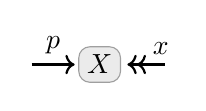
\begin{tikzpicture}[center base]
		\node[dpad0] (X) {$X$};
		\coordinate (A) at ($(X) + (-0.9,0)$);
		\draw[arr1] (A) -- node[above]{$p$}  (X);
%
		\draw[arr2, <<-] (X) --  node[above,pos=0.8]{$x$} ++(0.9, 0);
	\end{tikzpicture}
	}.
	\]
\end{linked}
%joe1*: Again, SLOW DOWN and helpe the reader by explaining what the
%PDG is saying

In some ways, this result is entirely unsurprising, given that PDG inconsistency \eqref{eq:inc} is a flexible formula built out of information theoretic primitives.
%
Even so, it is worth noting that
% With a little more focus on the context and less on the algebra, perhaps \Cref{prop:pdg-Ix} becomes more curous:
the inconsistency of the PDG containing just a distribution $p(X)$ and
a sample $x$ happens to be the standard relationship between a
%joe1
%distribution $p$ and sample $x$ --- and it is even known known as
distribution $p$ and sample $x$---and it is even named after
%joe1*: the notion of "cognitive dissonance" has a lot of baggage that
%comes with it (Festinger's experiments).  I doubt that most
%psychologists would associate surprise with cognitive dissonance.  I
%woujld *strongly* recommend that you don't bring it up here, unless
%you can make a much better connectin.
%``surprise'', a particular kind of cognitive dissonance.
%oli1: I'll use different words then:
% ``surprise''.
``surprise'', a certain expression of epistemic conflict.

% For this argument to be pesuasive, one needs to accept our definition of inconsistency more broadly. \Cref{prop:pdg-Ix} is a very simple special case.
% One concern is that it does not model the whole state of affairs; we train probabilstic models models with more than one sample.
Still, we have a ways to go before this amounts to any more than a curiosity.
One concern is that this picture is incomplete; we train probabilstic models models with more than one sample.
What if we replce $x$ with an empirical distribution on many samples?
% The first step in the proof of \cref{prop:pdg-Ix} is no longer valid, but we can get the same effect by being extremely confident in the data distribution.
\begin{linked}{prop}{expected-surprise}
	% Given a model 
    % determining a probability distribution with mass function 
	If 
	%joe1: what do you mean by "model" here.  Can you nsut say that p(X)
	%is a distribution on X.
	%%oli1: yes, but my audience here is people who use cross-entropy, and might not
	%% think of their generative models as probabilisty distributions without prodding. Try this:
    % $p(X)$ is a model,
    $p(X)$ is a probabilistic model of $X$,
	and $\xsamp = \{ x_i \}_{i=1}^m$ are samples
    with empirical distribution $\datadist\xsamp$, then 
	~~~$\mathrm{CrossEntropy}(\datadist\xsamp, p) = $
    %
    \begin{align*}
        \frac{1}{m} \sum_{i=1}^m \I_p(x_i) &=
        \aar[\Big] {
		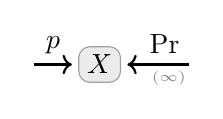
\begin{tikzpicture}[center base]
			\node[dpad0] (X) {$X$};
			\coordinate (A) at ($(X) + (-0.9,0)$);
			\draw[arr2] (A) -- node[above]{$p$}  (X);
			\draw[arr2, <-] (X) --  
                node[above,pos=0.6,inner sep=2pt]{${\datadist\xsamp}$}
                node[below,pos=0.65,inner sep=2pt]
                    {${\color{gray}\scriptscriptstyle(\infty)}$}
             ++(1.2, 0);
				%\overset{\{\beta = \infty\}}
		\end{tikzpicture}
		}%_\gamma
        %
		%joe1*: putting this in gray is distracting and makes it harder to
		%read.  I see no benefit.        
		%oli1: Fiiiiine, I begrudingly accept the standard
		% ~{\color{gray}+ \H(\datadist\xsamp)}.
		~{+ \H(\datadist\xsamp)}
        % \\
        % &= \mathrm{CrossEntropy}(\datadist\xsamp, p).
	\end{align*}
% 	\begin{enumerate}
% 	\item The average negative log likelihood $\ell(p; \xsamp) = - \frac{1}{m} \sum_{i=1}^m \log p(x_i)$
% 	\item The cross entropy of $p$ relative to $\datadist\xsamp$
% 	\item $\bbr{\,p\,}_\gamma(\datadist\xsamp) ~{\color{gray}~+ (1+\gamma)\H(\datadist\xsamp)}$ \\[-1.4em]
% 	% FALSE! \item $\bbr{\,p^{\{\alpha=1\}} \,}_1 (\datadist\xsamp^{\{\alpha=1\}})$
% 	\item
% 	% \item
% 	% \(\aar[\Bigg] {
% 	% 	\begin{tikzpicture}[center base]
% 	% 		\node[dpad0] (X) {$X$};
% 	% 		\coordinate (A) at ($(X) + (-1.2,0)$);
% 	% 		\draw[arr1] (A) -- node[above,pos=0.4]{$ \overset {\{\alpha = 1\}} p$}  (X);
% 	% %
% 	% 		\draw[arr2, <-] (X) --  node[above,pos=0.6]{$ \overset{\{\beta = \infty,\alpha=\gamma\}}{\datadist\xsamp}$} ++(1.5, 0);
% 	% 	\end{tikzpicture}
% 	% 	}\!\bigg._1 \)
% \end{enumerate}
\end{linked}
\begin{remark}
	%oli1:
	% Note that the entropy of the data distribution $\H(\datadist\xsamp)$
	The term $H(\datadist\xsamp)$
	%joe1: If this is your reason for putting it in gray, it's a bad one
	%does not depend on $p$, and so the final grey term is irrelevant for
	%oli1: ok. rewording since I've already given the formula.
	% does not depend on $p$, and so the $\H(\datadist\xsamp)$ term is irrelevant for finding $p$ to minimize it. 
	% does not depend on $p$, and hence is irrelevant for 
	is a constant depending only on the data, so is irrelevant for optimizing $p$.
\end{remark}

% The PDG in  \cref{prop:expected-surprise} is quite natural.
% Aside from the certainty weights $\beta$, we've simply translated each piece of information into a cpd, and collected them together as a PDG.
% We argue that the choice of $\beta$ makes sense as well, in the standard use cases for  cross entropy / log likelihood.
% % In the current setting, we argue that the weights are also the ones we would expect.
% The cross entropy measures the expected code length per sample, when a (possibly incorrect) distribution $p$ is used to design a code, in place of the true one $\datadist\xsamp$.
% So implicitly, a modeler who chooses a cross-entropy has in some sense implicitly articulated a belief the data distribution is the ``true one'', by placing infinite certainty in $\datadist\xsamp$ than in $p$.
% If $p(X)$ represents a probabilistic model before training is complete (say, a neural network with randomly initialized weights), we would be justified in placing dramatically more trust in the data $\datadist\xsamp$ than in $p$, and so this choice seems particularly appropriate.
% % This justifies the `!'.
% Other choices of $\beta$ are natural in other contexts, and we will see in \cref{sec:statdist} that they correspond to other losses. (For instance when $\beta_p = \beta_{\datadist\xsamp} = \nicefrac12$, the result is the Bhattacharyya distance, rather than the cross entropy.)
The only choice we've made in specifying the PDG of \cref{prop:expected-surprise} are the confidences.
But $\mathrm{CrossEntropy}(\datadist\xsamp,p)$ is the expected code length per sample
from $\datadist\xsamp$, when using codes optimized for the (incorrect) distribution $p$.
% TODO fixme. DO I need Citation? Also, this is perhaps not the best 
% citation for the claim. 
% \parencite{shore1980relent}.
So implicitly, a practitioner using cross-entropy has already articulated a belief the data distribution is the ``true one''. 
To get the same effect from a PDG, the modeler must make this belief explicit by placing infinite certainty in $\datadist\xsamp$. 

We now consider an orthogonal generalization of \cref{prop:pdg-Ix}, in which the sample $x$ is only a partial observation of a joint model $p(X,Z)$. In this case, we might hope to recover the \emph{marginal} surprise, since $Z$ does not interact with the observation. % ---  in \cref{prop:marginal-ll}.

\begin{linked}{prop}{marginal-ll}
	If $p(X,Z)$ is a joint distribution, the information content of the partial observation $X=x$, or the marginal negative log likelihood of $x$, is given by
	\begin{equation}
	 	\I_p(x) = \log \frac{1}{p(x)} =
	    % \lim_{t \to \infty}
		 \aar[\Bigg]{
	% 	  \Inc\left(
			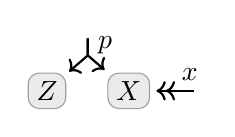
\begin{tikzpicture}[center base]
				\node[dpad0] (Z) {$Z$};
				\node[dpad0,right=.5 of Z] (X) {$X$};
				\coordinate (A) at ($ (X)!.5!(Z) + (0,0.7)$);
				\draw[arr1] (A) -- node[right]{$ p$} ++(0,-0.25) -- (X);
				\draw[arr1] (A) -- ++(0,-0.25) -- (Z);
	%
				\draw[arr2, <<-] (X) --  node[above,pos=0.8]{$ x$} ++(0.9, 0);
	% 			\draw[arr2, <-] (Z) -- node[above,pos=0.6]{$ q^{\{\beta =\infty\}}$} ++(-0.9, 0);%
				% \ar[r,"p"] \& Z \ar[r,"p", bend left] \& X \ar[l,"q", bend left] \& \ar[l, two heads, "x"']
			\end{tikzpicture}
			}.
			\label{eq:mll}
	\end{equation}
\end{linked}

Intuitively, the inconsistency in the PDG on the right hand side of \eqref{eq:mll} is localized to $x$, where the sample conflicts with the distribution; other variables don't make a difference.
The natural generalization with both partial observations and multiple samples also holds, and we defer treatment to the appendix.
% Just as \cref{prop:expected-surprise} generalizes \cref{prop:pdg-Ix}, there is 
% a multi-sample analogue of analog of \Cref{prop:marginal-ll} .
% Furthermore, $p$ is the qualitative model we have in mind, and so we set $\alpha_p = 1$
 % by considering more than one sample at once, 



% So far we have been considering models of a distribution $p(X)$ that correspond to generative models, or an unsupervised setting.
So far we have considered models of an unconditional distribution $p(X)$.
% TODO
%joe1: you need a reference for the material below
% Because one can use such a model to generate samples, such models are called \emph{generative}, and their training process is called \emph{unsupervised} learning.
Because they are unconditional, such models must describe how to generate a complete sample $X$ without input, and so are called \emph{generative}, and the process of training them is called \emph{unsupervised} learning.
Contrast this with the (perhaps more common) \emph{supervised} setting, in which we train \emph{discriminative} models to predict $Y$ from $X$, from labeled samples ($X,Y$).
For supervised learning, cross entropy loss is perhaps even more dominant---and it equals the inconsistency of a PDG consisting of the predictor $f(Y|X)$ together with high-confidence data.

\begin{linked}{prop}{supervised-cross-entropy}
	% Consider a probabilistic model $f$ with mass function $f(Y \mid X)$. The inconsistency of the PDG containing $f$ and the empirical distribution $\datadist\xysamp$ of samples $\xysamp$ is equal to the negative log-liklihood (cross-entropy) loss, plus the empirical uncertainty in $Y$ given $X$ (a constant independent of $f$). That is,
    Consider a probabilistic predictor $f(Y \mid X)$. The
    inconsistency of the PDG containing $f$ and the empirical
	%joe1: is this standard notation for a set of samples?  I don't believe that
	%I've seen it before.  If it's not standard, you have to example it better
	%    distribution $\datadist\xysamp$ of samples $\xysamp$ is equal to
	%oli1: I'll expand
    % distribution $\datadist\xysamp$ of a set $\xysamp$ of samples is equal to
    distribution $\datadist\xysamp$ of a sample set $\xysamp = \{(x_i, y_i)\}_{i=1}^{m}$ is equal to
    the cross-entropy loss (minus the empirical uncertainty in $Y$
    given $X$, a constant that depends only on the data). That is, 
	\[ \aar**{
		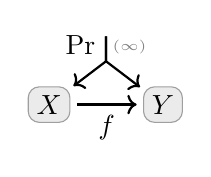
\begin{tikzpicture}[center base]
			\node[dpad0] (Y) {$Y$};
			\node[dpad0,left=.9 of Y] (X) {$X$};
			\coordinate (A) at ($ (X)!.5!(Y) + (0,0.9)$);
			%joe1*: you're back to using hte exclamation point notation, which you
			%never defined.  I *strongly* suggest that you get rid of it.  Pity
			%the poor reader!
			%oli1: oops. Missed this one.
			\draw[arr1] (A) --
				% node[right]{$\datadist\xysamp!$} 
				node[left,inner sep=3pt]{$\datadist\xysamp$} 
				node[right,inner sep=2pt]{${\color{gray}\scriptscriptstyle(\infty)}$} 
				++(0,-0.35) -- (X);
			\draw[arr1] (A) -- ++(0,-0.35) -- (Y);
			\draw[arr2, ->] (X) --  node[below,pos=0.5]{$f$} (Y);
		\end{tikzpicture}}
        \begin{aligned}
			%oli1: This should be clearer also.
            % \frac1{|\xysamp|}\sum_{(x,y) \in \xysamp} \left[ \log \frac1{f(y \mid x)}\right]&\\
            = \frac1{m}\sum_{i=1}^m \log \frac1{f(y_i\,|\, x_i)}&\\
             - \H_{\datadist\xysamp}(Y | X)&.
        \end{aligned}
	\]
\end{linked}

\begin{remark} \label{remark:continuous}
% \cref{prop:pdg-Ix,prop:expected-surprise,prop:marginal-ll,prop:pdg-loglikelihood,prop:supervised-cross-entropy} all require the probability to have a mass function, rather than a density function, which implicitly restricts us to discrete variables.
% \cref{prop:pdg-Ix,prop:expected-surprise,prop:marginal-ll,prop:pdg-loglikelihood,prop:supervised-cross-entropy} 
Many of our results require the distribution to be represented with a mass function (not a density function (pdf)).
%joe1*: We've never talked about the inconsistency of a continuous
%distribution.  If it's always infinite, this suggests that whatever
%definition you have in mind is not good.  I would strongly suggest
%that you deal with onoly discrete distributions here.  If you venture
%into continuous distributions, you *must* explain inconsistency for
%them better, and motivate it.   You can instead just talk about
%approximating the continuous distrbution by a discrete
%distribution. or perhaps a distribution that takes on only finitely
%many values.  
A PDG containg both pdf and a finitely supported distribution on the same variable
will typically have infinite inconsistency. 
%joe1*: I fell off the cliff in the next few sentences.  I strongly
%suggest you cut them (which you can do if you say that you're just
%considering discrete distributions.
This is not just a quirk of the PDG formalism.
% of the standard objectives. 
The analog of surprisal for a density $p(X)$ is problematic because probability density is not dimensionless (like probability mass), but rather has inverse $X$-units (e.g., probability per meter), so depends on an arbitrary choice of scale (the pdf for probability per meter and per centimeter will yield different numbers).
%
That said, a rescaling ultimately only adds a constant.
% Similarly, any approximation of a density $p(X)$ with a discretization $\tilde p_k(X)$ where $k$ discretization size, differs only
Moreover, refining the discretization size $k$ of a discretized approximation $\tilde p_k(X)$ also contributes a constant that depends only on $k$.
    % \cref{prop:pdg-Ix,prop:expected-surprise,prop:marginal-ll,prop:pdg-loglikelihood,prop:supervised-cross-entropy}
% only in a constant that depends only on $k$.
% But this constant is irrelevant for optimization, justifying the use of the continuous analogues (such as $- \log p(x)$ for a pdf $p(x)$) as loss functions.
Such constants are irrelevant for optimization, justifying the use of the continuous analogues as loss functions.
%TODO.
\end{remark}

\subsection{Simple Performance Metrics as Inconsistencies}

There are also simpler scoring metrics used to evaluate the performance of systems on datasets, such as the accuracy of a  classifier, or the mean-squared error of a regressor. These too naturally arise as inconsistencies.

\begin{linked}[log accuracy as inconsistency]
		{prop}{accuracy}
	% If $h: X \to Y$ is a predictor for an input space $X$ and label space $Y$, and $f: X \to Y$ generates the correct labels, then the inconsistency of believing $f$ and $h$ (with any degree of confidence), and also that inputs are distributed according to $D(X)$, equals the information content of learning that $f(X) = h(X)$ according to $D$ (which is the log accuracy of the predictor $h$) times the confidence in $D$. That is,
	%joe1: You've been writing p(X).  Why suddenly switch to D(x)                
	%    Consider $D(X)$ over inputs $X$, and functions $f,h : X \to Y$,
	%oli1: ... because this was more the anlog of $\Pr$, but I didn't want to insist on
	% an emperical distribution over samples. I think maybe just $\Pr$ with no subscript
	% is clearer, but it makes me slightly unhappy because then $\Pr$ isn't just a function
	% from models to probability distributions anymore.
	%TODO
    Consider a distribution $D(X)$ over inputs $X$, and functions $f,h
    : X \to Y$, 
                where $h$ is a predictor and $f$ generates the true labels. The
    inconsistency of believing all three is: 
	\begin{equation}\label{eq:accuracy-pdg}
		\aar*{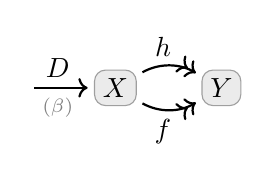
\begin{tikzpicture}[center base]
				\node[dpad0] (Y) {$Y$};
				\node[dpad0,left=0.8 of Y] (X) {$X$};
				%
				\draw[arr2, ->>] (X) to[bend left] node[pos=0.4, above]{$h$} (Y);
				\draw[arr2, ->>] (X) to[bend right] node[pos=0.4, below]{$f$} (Y);
				\draw[arr2, <-] (X) to
                    node[pos=0.55, anchor=south west, above]
					% {$\overset{(\beta)}D$} +(-1.1, 0);
					% {$D^{\color{gray}(\beta)}$}
                    {$D$}
                    node[pos=0.55, anchor=south west, below]
                    {{\color{gray}$\scriptstyle(\beta)$}}
                    +(-1.1, 0);
			\end{tikzpicture}}
        \begin{aligned}
		% &=  - \beta\,\log \Big( \mathrm{accuracy}_{f,D} (h) \Big) \\
		&=  - \beta\,\log \Pr_{x \sim D}(f(x) = h(x))  \\
		&\quad= \beta\, \I_D [f = h].
        \end{aligned}
	\end{equation}
\end{linked}
%joe1*: you need to give a reference for all this, and to discuss
%accuracy and what it's capturing *before* you state the theorem.  
%TODO
It is common to think of accuracy as a property of a hypothesis $h$
(with some dependence on the true labeling function $f$ and the data
distribution $D$), even though it is symmetric in $f$ and $g$, in part
because we change the predictor more than the labels. 
The correspondence of \Cref{prop:accuracy} graphically depicts this symmmetry, and also a more subtle phenomenon: a particularly strong dependence on the distribution of inputs.
In fact, the inconsistency of the PDG in \eqref{eq:accuracy-pdg} is scaled by the confidence of $D$, but does not depend at all on the confidences in $h$ or $f$.

Why should this be the case? The deterministic nature of $f$ and $h$ encodes extreme confidence (to anthropomorphise: $f$ thinks it impossible that $Y \ne f(X)$, because that event has probability zero), and so the only way to selectively choose samples to make things consistent is to alter the distribution of \emph{inputs} $\Pr(X)$ (so that it is always the case that $f(x) = g(x)$), not to change $\Pr(Y|X)$.
But it is the direction that we want to pull $\Pr(Y| X)$ that
informs how we should update our predictor $h(Y\,|\,X)$, which
%joe1*: Where did non-differentiability come from?  This is totally
%out of the blue.    You should fget rid of it.
%TODO
reflects the non-differentiability of the accuracy (or zero-one loss)
with respect to $h$. 
Note that this is the \emph{exact opposite} of how we captured cross entropy (\cref{prop:supervised-cross-entropy}), in which we are unwilling to budge on the data distribution, but are willing to modify our predictor $h$.



% \begin{prop}[Cosine similarity as inconsistency]
% 	\todo
% \end{prop}
%% Confusion matrix costs
% \begin{prop}
% 	\[
% 	\]
% \end{prop}


When $Y$ is continuous rather than discrete, the estimator is referred
to as a regressor instead of a classifier, and the newfound topology
of $Y$ suggests that some mistakes are worse than others---that we
might want to treat a small deviation from the correct value of $Y$.
%TODO
%joe1*: this is a nonsequitur from the egnning of the paragraph.
%Also, what does it mean that f and h "control" the mean of a
%Gaussian?  Do you mean that they determine some parameters of the
%Gaussian?  If so, you should say that.
Perhaps the most common way of measuring this deviation is with mean
square error, which corresponds to the inconsistency of believing that
%joe1
%$f$ and $h$ control the mean of a unit-variance gaussian.
$f$ and $h$ control the mean of a unit-variance Gaussian. 

\begin{linked}[square error as inconsistency]{prop}{MSE}% \label{coro:MSE}
	\begin{align*}
		% \aar**{\begin{tikzpicture}[center base]
		% 	\node[dpad0] (Y) {$Y$};
		% 	\node[dpad0,left=1.1 of Y] (X) {$X$};
		% 	%
		% 	\draw[arr2, ->] (X) to[bend left]
		% 		node[pos=0.5, above] {$\mathcal N(f(x), 1)$} (Y);
		% 	\draw[arr2, ->] (X) to[bend right] node[pos=0.5, below]{$\mathcal N(g(x), 1)$} (Y);
		% 	\draw[arr2, <-] (X) to node[pos=0.6, above]{$D!$} +(-1.1, 0);
		% \end{tikzpicture}}
		% &=
		\aar**{\!\!\!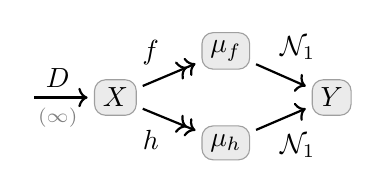
\begin{tikzpicture}[center base]
			\node[dpad0] (Y) {$Y$};
			\node[dpad0,left=2.2 of Y] (X) {$X$};
			\node[dpad0,above right=0.1 and 0.8 of X] (mf) {$\mu_f$};
			\node[dpad0,below right=0.1 and 0.8 of X] (mh) {$\mu_h$};
			%
			\draw[arr2, ->>] (X) to[bend left=0]
				node[pos=0.5, above left=0] {$f$} (mf);
			\draw[arr2, ->>] (X) to[bend right=0]
				node[pos=0.5, below left=0] {$h$} (mh);
			%
			% \draw[arr2, <-] (X) to node[pos=0.6, above]{$D!$} +(-1.1, 0);
			\draw[arr2, <-] (X) to
                node[pos=0.55, above] {$D$}
                node[pos=0.55, below]
                {{\color{gray}$\scriptstyle(\infty)$}}
                +(-1.1, 0);
			%
			\draw[arr2, ->] (mh) to[bend right=0]
				node[pos=0.3, below right=0] {$\mathcal N_1$} (Y);
			\draw[arr2, ->] (mf) to[bend left=0]
				node[pos=0.3, above right=0]{$\mathcal N_1$} (Y);
			% \draw[arr2, <-] (X) to node[pos=0.6, above]{$D$} +(-1.1, 0);
		\end{tikzpicture}\!\!}
		\begin{aligned}
        = \Ex\nolimits_D \!\big( f(X) - h(X) \big)^2 \\
		 = \mathrm{MSE}( f, h )~,~
        \end{aligned}
        %\numberthis\label{eq:mse}
	\end{align*}
	where
    % $\mathcal N_1 = \mathcal N(-,1)$
    $\mathcal N_1$
    % is the unit normal distribution with the given mean.
	is the unit-variance normal distribution with the given mean.
\end{linked}
%
We treat the more general case, with arbitrary variances and confidences, in the appendix.

%%%%%%%%%%%%%%%%%%%%%%%%%%%%%%%%%%%%%%%%%%
% The fact that $\mathrm{QM}(a, b) > \mathrm{GM}(a,b)$ for $a, b >0$ has been used to movivate a metric  between different power means is sometimes used to measure the
% \eqref{eq:2gaussians} and  gives
% \begin{equation*}
% \aar**{\begin{tikzpicture}[center base]
% 	\node[dpad0] (Y) {$Y$};
% 	%
% 	% \draw[arr2, ->] (X) to[bend left]
% 	% 	node[pos=0.5, above] {$\mathcal N(0, s(x))$} (Y);
% 	% \draw[arr2, ->] (X) to[bend right] node[pos=0.5, below]{$\mathcal N(0, t(x))$} (Y);
% 	\draw[arr2, <-] (Y) to node[pos=0.6, above]{$\mathcal N(0, \sigma_1)$} +(-1.4, 0);
% 	\draw[arr2, <-] (Y) to node[pos=0.6, above]{$\mathcal N(0, \sigma_2)$} +(1.4, 0);
% \end{tikzpicture}}
% =  \log
% 	 \frac
% 	 {\mathrm {QM}(\sigma_1,\sigma_2)}
% 	 {\mathrm {GM}(\sigma_1,\sigma_2)}
% \end{equation*}




% % The results in this section may not teach us very much that we did not know before, but
% Although the results in this section are not particularly useful on their own,
% they do display at a surprisingly strong tie between the standard metrics used to train probabilistic models, and the inconsistency of a corresponding PDG ---
% we have seen that (marginal) log likelihood, cross entropy, and log accuracy all arise naturally as inconsistencies of the appropriate PDGs.


%%%%%%%%%%%%%%%%%%%%%%%%%%%%%%%%%%%%%%%%%%%%%%%%%%%/%%%%%%%%%%%%%%%%%%%%%%
\section{STATISTICAL DISTANCES AS INCONSISTENCIES} \label{sec:statdist}
Suppose you are concerned with only a single variable $X$. One friend has told you that it is distributed according to the probability distribution $p(X)$; another has told you that it follows $q(X)$, and you adopt both beliefs. Your mental state will be inconsistent if (and only if) $p \ne q$, with more inconsistency the more $p$ and $q$ differ.
Thus the inconsistency of a PDG comprising $p$ and $q$ is a measure of divergence.

Recall that a PDG also allows us to specify the confidences $\beta_p$
%joe1
%and $\beta_q$ of each cpd, and so we can form a distinct PDG
and $\beta_q$ of each cpd, and so we can form a PDG
containing only $p(X)$ and $q(X)$ for each setting of
$(\beta_p, \beta_q)$. 
It turns out that a large classs of statistical distances are inconsistencies of such a PDG.
We start with one we've already seen.

\begin{prop}[KL Divergence as Inconsistency]
	The inconsistency of believing $p$ with complete certainty, and also $q$ with some finite certainty $\beta$, is $\beta$ times the KL Divergence (or relative entropy) of $q$ with respect to $p$. That is,
\vspace{-0.7em}
\[
    \aar[\Big]{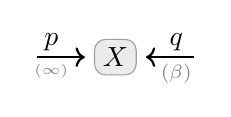
\begin{tikzpicture}[center base]
        \node[dpad0] (X) {$X$};
        \draw[arr, <-] (X) -- 
            node[above,inner sep=2pt, pos=0.65] {$p$}
            node[below,inner sep=2pt, pos=0.65] 
                {${\color{gray}\scriptscriptstyle(\infty)}$}
             ++(-1.1,0);
        \draw[arr, <-] (X) --  
            node[above,pos=0.6,inner sep=2pt]
            % {$\overset{\smash{\color{gray}(\beta)}}q$} ++(0.9, 0);
         	% {$\overset{{\color{gray}(\beta)}}q$}
            % {$q~^{{\color{gray}(\beta)}}$} ++(1.1, 0);
			{$q$}
			node[below,pos=0.6,inner sep=2pt]
                {$\scriptstyle{\color{gray}(\beta)}$}++(1.1, 0);
    \end{tikzpicture}}
	= \beta\, \kldiv pq .
\]
\end{prop}
This result gives us an intuitive interpretation of the asymmetry of relative entropy / KL divergence, and a prescription about when it makes sense to use it.
$\kldiv p q$ is the inconsistency of a mental state containing both $p$ and $q$, when absolutely certain of $p$ (and not willing to budge on it).
This concords with the standard view that $\kldiv pq$ reflects the amount of information required to change $q$ into $p$, which is why we call it the relative entropy ``from $q$ to $p$''.


% In general, we derive the following form for the inconsistency of a PDG whose contents are distributions $p(X)$ and $q(X)$, for arbitrary confidences.
We now consider the general case of a PDG comprising $p(X)$ and $q(X)$ with arbitrary confidences.
%, which we denote $\thickD^{PDG}_{r,s}(p,q)$,  .
\begin{linked}{lemma}{pdgdiv}
	% The PDG divergence $\thickD^{\mathrm{PDG}}_{(r,s)}(p, q)$,
    The inconsistency of a PDG containing $p(X)$ with confidence $r$ and $q(X)$ with confidence $s$
    is given in closed form by
    \[
		% \thickD^{\mathrm{PDG}}_{(r,s)}(p, q) :=
        \aar[\bigg]{\!\!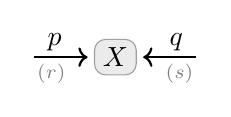
\begin{tikzpicture}[baseline = -0.75ex]
            \node[dpad0] (X) {$X$};
            \draw[arr2, <-] (X) --
			 		% node[above] {$\overset{(\beta : r)}p$}
			 		node[above, pos=0.6, inner sep=2pt, align=center] {$p$}
			 		node[below, pos=0.65, inner sep=2pt, align=center]
                        % {$\scriptstyle{\color{gray}(\beta : r)}$}
                        {$\scriptstyle{\color{gray}(r)}$}
				++(-1.1,0);
            \draw[arr2, <-] (X) --
					% node[above,pos=0.5] {$\overset{(\beta : s)}q$}
			 		node[above, pos=0.6, inner sep=2pt, align=center] {$q$}
			 		node[below, pos=0.65, inner sep=2pt, align=center]
                        % {$\scriptstyle{\color{gray}(\beta : s)}$}
                        {$\scriptstyle{\color{gray}(s)}$}
				 ++(1.1, 0);
        \end{tikzpicture}\!\!}
        % = \thickD^{\mathrm{PDG}}_{(r,s)}(p, q)
        = - (r+s) \log  \sum_x \left(p(x)^{r}\vphantom{\Big|} q(x)^{s}\right)^{\frac{1}{r+s}}.
        % = - (r+s) \log \sum_x \! \sqrt[\leftroot{0}\uproot{2}r+s]{\vphantom{\big|}p(x)^{r} q(x)^{s}}
    % \qquad\text{where}\qquad \xi:= \beta_p+\beta_q
    \]
\end{linked}


\begin{figure*}
	\centering
	\def\ptradius{0.07}
	\begin{tikzpicture}[xscale=1.8, yscale=1.4]\def\rotateangle{39}
		% \draw[help lines, color=gray!30, dashed] (-0.9,-1.4) grid (5.9,2.9);
		% \draw[->,thick] (-1,0)--(6,0) node[right]{$\beta_p$};
		% \draw[->,thick] (0,-1.5)--(0,3) node[above]{$\beta_q$} ;

		\draw[help lines, color=gray!30, dashed] (-1.2,-1.1) grid (5.9,2.7);
		\draw[->,thick] (-1.3,0)--(6,0) node[right]{$\beta_p$};
		\draw[->,thick] (0,-1.2)--(0,2.8) node[above]{$\beta_q$} ;

		%concave part
		% \fill[gray, fill opacity=0.2] (-1,1) -- (1.5,-1.5) -- (-1,-1.5) --cycle;
		\fill[gray, fill opacity=0.2] (-1.3,1.3) -- (1.2,-1.2) -- (-1.3,-1.2) --cycle;
		\draw[gray, opacity=0.5, thick] (-1.3,1.3) --
		node[below left=0.5em and 1.5em, anchor=north, rotate=-\rotateangle,font=\footnotesize,fill=gray!20,fill opacity=0.8, inner sep=1pt, outer sep=3pt] % at (-0.5,-0.5)
			% {Non-convex region} (1.5,-1.5);
			{Non-convex region} (1.2,-1.2);
		%axis of symmetry
		% \draw[color=orange!25, thick] (-1, -1) -- (3,3);
		% \fill[orange, opacity=0.05] (-1,-1) -- (3,3) -- (-1,3) -- cycle;
		\draw[color=gray!80!orange!45, densely dashdotted] (-1, -1) -- (3,3);
		% \draw[color=gray!80!orange!45, thick, <->] (2.8, 2.2) -- node[above right, anchor=south, rotate=-\rotateangle,font=\footnotesize,fill=white,fill opacity=0.8, inner sep=1pt, outer sep=3pt]{Axis of Symmtry}(2.2,2.8);
		\draw[color=gray!80!orange!45, thick, <->] (1.8, 1.2) -- node[above right, anchor=south, rotate=-\rotateangle,font=\footnotesize,fill=white,fill opacity=0.8, inner sep=1pt, outer sep=3pt]{\scalebox{0.8}{Axis of Symmtry}}(1.2,1.8);


		% Renyi Entropy Line
		\draw[blue!40, densely dashed, very thick, opacity=0.8]
		 	(0,1) -- node[below, align=center, pos=0.8, font=\footnotesize]{R\'enyi divergences\\for $\alpha \in (0,1)$} (5.6,1)
			(5.6,-1) -- node[above, align=center, pos=0.2, font=\footnotesize]{(negative) R\'enyi divergences\\ for $\alpha \in (1,\infty)$} (1,-1);
		%Chernoff Information Line
		\draw[red!90!blue!40, densely dashed, very thick, opacity=0.9, (-), shorten <=6pt, shorten >=6pt]
		 	(0,1) -- 
            node[pos=0.5,below left=3pt,anchor=north, rotate=-\rotateangle, font=\footnotesize, align=center, fill=white,fill opacity=0.8, inner sep=1pt, outer sep=2pt]
                {\scalebox{0.9}{Chernoff}} 
            node[pos=0.5,below left=1.25em,anchor=north, rotate=-\rotateangle, font=\footnotesize, align=center, fill=white,fill opacity=0.8, inner sep=1pt, outer sep=2pt]{\scalebox{0.9}{Divergences}}
            (1,0);
		%alpha divergence line
		% \draw[domain=1.5:5.6, smooth, very thick, variable=\x, blue!50!green!50, opacity=0.8, densely dashed] plot ({\x}, {1/(1-1/\x)})
		\draw[domain=1.6:5.6, smooth, very thick, variable=\x, blue!50!green!50, opacity=0.8, densely dashed] plot ({\x}, {1/(1-1/\x)})
			node[rotate=-7, font=\footnotesize] at (3.9,1.55){$\alpha$-divergences};

		%%%% POINTS %%%%
		%[draw, very thick,fill=magenta!50!black]
		\fill (0.5,0.5) circle (\ptradius) node[above right, align=center,
			label={[yshift=0ex,xshift=-1ex,align=left,font=\footnotesize\color{gray!50}]right:Bhattacharya\\distance}]
			% {Bhattacharya\\distance};
			% {$\thickD^{\text{Bhattacharya}}$};
			{$\thickD_{B}(p,q)$};

		% \fill (1,3.4) -- +(0:\ptradius) arc (0:-180:\ptradius) -- +(0:\ptradius)
		% 	node[below]{$\vdots$}
		% 	node[right=1ex, align=center,label={[yshift=1ex,xshift=0ex]below:\footnotesize\color{gray!50}Reverse KL}](revKL){$\kldiv qp$};
		\fill (1,3.1) -- +(0:\ptradius) arc (0:-180:\ptradius) -- +(0:\ptradius)
			node[below]{$\vdots$}
			node[right=1ex, align=center,label={[yshift=1ex,xshift=0ex]below:\footnotesize\color{gray!50}Reverse KL}](revKL){$\kldiv qp$};
        
		\fill (6.4,1) -- +(270:\ptradius) arc (270:90:\ptradius) -- +(270:\ptradius)
			node[above=2pt, align=center,
				label={[yshift=-1ex,xshift=0ex]\footnotesize\color{gray!50} KL Divergence}] (FwdKL) {$\kldiv pq$}
			node[left]{$\cdots$};

		\fill (0,1) -- ++(-90:\ptradius) arc (-90:90:\ptradius)
			node[above right, align=center,
				label={[yshift=-1ex,xshift=1ex]\footnotesize\color{gray!50} Max Entropy}
			]{$\I_q(p > 0)$};

		% divergences requiring negative \beta
		% \fill (2,-1) circle (\ptradius) node[below right, align=center,
		% 		label={[yshift=1ex,xshift=1ex]below:\footnotesize\color{gray!50}$-\chi^2$ divergence}]
		% 	{$-\chi^2\infdivx pq$};
        \fill (2,-1) circle (\ptradius) 
            node[above right, align=center,
                label={[yshift=-1ex,xshift=1ex, align=center,font=\footnotesize\color{gray!50}]above:$-$(Pearson)~$\chi^2$ \\[-0.1em]divergence}]
            {$-\chi^2_P\infdivx pq$};
        
        \fill (-1,2) circle (\ptradius) 
            node[above, align=center,
                label={[yshift=-1ex,xshift=1ex, align=center,font=\footnotesize\color{gray!50}]above:$-$(Neyman)~$\chi^2$ \\[-0.1em]divergence}]
            {$-\chi^2_N\infdivx pq$};
            
		\fill (1,-1) -- ++(-45:\ptradius) arc (-45:135:\ptradius)
			node[above, align=center, inner sep=2pt,
				label={[yshift=-1ex,xshift=1ex]\footnotesize\color{gray!50} $-$Min Entropy}]
			{$- \log \sup \frac pq$};



	\end{tikzpicture}
	\caption{A map of the inconsistency of the PDG comprising $p(X)$ and $q(X)$, as we vary their respective confidences $\beta_p$ and $\beta_q$. Solid circles indicate well-known named measures, semicircles indicate limiting values, and the heavily dashed lines are well-established classes. }
	% {A map of inconsistency
	% \(\aar[\bigg]{\begin{tikzpicture}[center base]
	% 	\node[dpad0] (X) {$X$};
	% 	\draw[arr2, <-] (X) --
	% 			node[above, pos=0.6, inner sep=2pt, align=center] {$p$}
	% 			node[below, pos=0.65, inner sep=3pt, align=center] {$\scriptstyle{\color{gray}(\beta_p)}$}
	% 		++(-1.1,0);
	% 	\draw[arr2, <-] (X) --
	% 			node[above, pos=0.6, inner sep=2pt, align=center] {$q$}
	% 			node[below, pos=0.65, inner sep=3pt, align=center] {$\scriptstyle{\color{gray}(\beta_q)}$}
	% 		 ++(1.1, 0);
	% \end{tikzpicture}}\)
	% as we vary the confidences $(\beta_p, \beta_q)$ in the distributions $p$ and $q$. }
	\label{fig:statdistmap}
\end{figure*}




Of the many generalizations of KL divergence, R\'enyi divergences, first characterized by Alfr\'ed R\'enyi \citeyear{renyi1961measures} are perhaps the most significant, as few others have found either application or an interpretation in terms of coding theory \parencite{van2014renyi}.
The R\'enyi divergence of order $\alpha$ between two distributions $p(X)$ and $q(X)$ is given by
\begin{equation}
	\thickD_\alpha\infdivx p q := \frac{1}{1- \alpha} \log \sum_{x \in \V(X)} p(x)^\alpha q(x)^{1-\alpha}.  \label{eq:renyi}
\end{equation}
R\'enyi introduced this measure in the same paper as the more general
class of $f$-divergences, but directs his attention towards those of
%joe1
%the form \eqref{eq:renyi}, because satisfy a natural weakening of
%Fadeev's postulates \cite{fadeev1957begriff}, for Shannon entropy.
the form \eqref{eq:renyi}, because they satisfy a natural weakening of
standard postulates for Shannon entropy due to 
% Fadeev \citeyear{fadeev1957begriff}.
\textcite{fadeev1957begriff}.
Concretely, every symmetric, continuous measure that additively separates over independent events, and with a certain ``mean-value property'', up to scaling, 
% is a R\'enyi divergence \eqref{eq:renyi} for some $\alpha$, up to scaling \cite{renyi1961measures}.
is of the form \eqref{eq:renyi} for some $\alpha$ \parencite{renyi1961measures}.
%joe1: this needs a spellcheck
%It follows from \cref{lemma:pdgdiv} that varing the confidences of our
It follows from \cref{lemma:pdgdiv} that varying the confidences of our
two-distribution PDG, essentially carves out the same class: every
R\'enyi divergence is the inconsistency of some PDG of this form, and
every PDG divergence is a (scaled) R\'enyi
divergence. 

%joe1: you[r talk about Renyi entropy and Renyi divergence.  Do you
%mean entropy?
%oli1: The divergence is more general; I'll just refer to that for consistency.
\begin{coro}[R\'enyi Divergences]
	% xx
    % \vskip-1em
	~\vspace{-1ex}
    \begin{align*}%
        % \thickD^{\mathrm{PDG}}_{r, s}(p, q) 
        \aar[\Big]{\!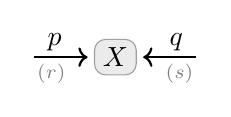
\begin{tikzpicture}[baseline = -0.75ex]
            \node[dpad0] (X) {$X$};
            \draw[arr2, <-] (X) --
			 		% node[above] {$\overset{(\beta : r)}p$}
			 		node[above, pos=0.6, inner sep=2pt, align=center] {$p$}
			 		node[below, pos=0.65, inner sep=2pt, align=center]
                        % {$\scriptstyle{\color{gray}(\beta : r)}$}
                        {$\scriptstyle{\color{gray}(r)}$}
				++(-1.1,0);
            \draw[arr2, <-] (X) --
					% node[above,pos=0.5] {$\overset{(\beta : s)}q$}
			 		node[above, pos=0.6, inner sep=2pt, align=center] {$q$}
			 		node[below, pos=0.65, inner sep=2pt, align=center]
                        % {$\scriptstyle{\color{gray}(\beta : s)}$}
                        {$\scriptstyle{\color{gray}(s)}$}
				 ++(1.1, 0);
        \end{tikzpicture}\!}
            &=
            s \cdot \thickD_{\frac{r}{r+s}}\infdivx{p}{q}
        % \qquad \text{and} \qquad
        \\[-0.3em]\text{and}\qquad
        \thickD_{\alpha}\infdivx{p}{q}
        &= 
        % \thickD^{\mathrm{PDG}}_{\left(\frac{\alpha}{1-\alpha}, 1\right)}(p, q).
        \aar[\Big]{\!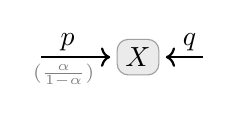
\begin{tikzpicture}[baseline = -0.75ex]
            \node[dpad0] (X) {$X$};
            \draw[arr2, <-] (X) --
			 		% node[above] {$\overset{(\beta : r)}p$}
			 		node[above, pos=0.6, inner sep=2pt, align=center] {$p$}
			 		node[below, pos=0.65, inner sep=2pt, align=center]
                        % {$\scriptstyle{\color{gray}(\beta : r)}$}
                        {$\scriptstyle{\color{gray}(\frac{\alpha}{1-\alpha})}$}
				++(-1.3,0);
            \draw[arr2, <-] (X) --
					% node[above,pos=0.5] {$\overset{(\beta : s)}q$}
			 		node[above, pos=0.6, inner sep=2pt, align=center] {$q$}
			 		% node[below, pos=0.65, inner sep=2pt, align=center]
                        % {$\scriptstyle{\color{gray}(\beta : s)}$}
                        % {$\scriptstyle{\color{gray}(s)}$}
				 ++(0.9, 0);
        \end{tikzpicture}\!}
    \end{align*}
\end{coro}

However, the two classes are not identical, because the PDG divergences admit extra limit points. One of the biggest differences is that the reverse KL divergence $\kldiv q p$ is not a Renyi entropy of the form $\thickD_\alpha\infdivx p q$ for any value (or limit) of $\alpha$. This lack of symmetry has caused other authors \parencite{cichocki2010families} to instead work with a re-scaled symmetric version of the R\'enyi entropy, called $\alpha$-divergence%
, which as an additional factor of $\frac1\alpha$.
% \eqref{eq:alphadiv}  (although sometimes the term is used for the same quantity without the logarithm).
The relationships between these quantities can be seen in \cref{fig:statdistmap}.

% \begin{equation}
% 	\tilde \thickD_\alpha\infdivx p q := \frac{1}{\alpha( 1- \alpha)} \;{\color{black}\log}\!\! \sum_{x \in \V(X)} p(x)^\alpha q(x)^{1-\alpha} \label{eq:alphadiv}
% \end{equation}
%
%% What is the point of this paragraph? CUT.
% We submit that viewing these as inconsistencies can clarify things a great deal. Whereas the formula for R\'enyi entropy is mostly symmetric, the leading $\frac1{1-\alpha}$ of \eqref{eq:renyi} makes it instead \emph{skew}-symmetric, and as a result the behavior for $\alpha \in (0, \nicefrac12)$ is qualitatively different from the behavior for $\alpha \in (\nicefrac12, 1)$.
% PDG inconsistency, on the other hand, is symmetric: the semantics do not give special treatment to one edge over the other.


The Chernoff divergence, measures the tightest possible exponential
bound on probability of error \parencite{nielsen2011chernoff} in Bayesian
%joe1
%hypotehsis testing.
hypothesis testing. 
It also happens to be the smallest possible inconsistency of simultaneously believing $p$ and $q$, with combined confidence 1.
\begin{coro}%[Chernoff Divergence as Inconsistency]
The Chernoff Divergence between $p$ and $q$ equals
\\[-1.8em]
% \vspace{-0.8em}
% \hfill
% \(
\[
	\inf_{\beta \in (0,1)}
	\aar[\Big]{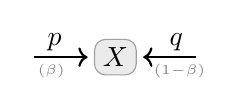
\begin{tikzpicture}[center base]
		\node[dpad0] (X) {$X$};
		\draw[arr2, <-] (X) --
			% node[above] {$\overset{(\beta)}p$}
			node[above, inner sep=2pt,pos=0.6] {$p$}
			node[below, inner sep=2pt,pos=0.65] {${\color{gray}\scriptscriptstyle(\beta)}$}
			 ++(-1.1,0);
		\draw[arr2, <-] (X) --
			% node[above,pos=0.5] {$\overset{(1-\beta)}q$}
			node[above, inner sep=2pt,pos=0.6] {$q$}
			node[below, inner sep=2pt, pos=0.65] {${\color{gray}\scriptscriptstyle(1-\beta)}$}
			++(1.1, 0);
	\end{tikzpicture}}.
	% = \thickD^{\mathrm{PDG}}_{(r,s)}(p, q)
	% = \thickD^{\text{Chernoff}}(p,q)
	% = - (r+s) \log \sum_x \! \sqrt[\leftroot{0}\uproot{2}r+s]{\vphantom{\big|}p(x)^{r} q(x)^{s}}
% \qquad\text{where}\qquad \xi:= \beta_p+\beta_q
\]
% \)
\end{coro}

One significant consequence of representing divergences as inconsistencies is that we can use \cref{lemma!} to derive relationships between them. The following facts follow from \cref{fig:statdistmap} by inspection.
\begin{coro}
	\begin{enumerate}[nosep]
		\item R\'enyi entropy is monotonic in its parameter $\alpha$.
		% \item $\kldiv P Q \ge 2 \thickD_B(P,Q) \le \kldiv Q P$
		\item $\kldiv p q \ge 2 \thickD_B(p,q) \le \kldiv q p$
		\item If $q(p > 0) < 1$ (i.e., $q \not\ll p$), then $\kldiv q p = \infty$
	\end{enumerate}
\end{coro}



Recall that these results are only for simple PDGs, which contain one variable and two distributions.
Inconsistency of general PDGs, is in some sense a vast generalization of the Renyi divergences to arbitrary structured objects.

\section{REGULARIZERS AND PRIORS}
\label{sec:regularizers}
Regularizers are extra terms added to loss funtions, which provide a source of inductive bias on model parameters. 
There is a well-known correspondence between using a regularizer and
doing maximum \emph{a posteriori} inference with a prior,%
\footnote{A more detailed account can be found in the appendix}
% \parencite{williams1995bayesian,rennie2003l2,probinterpblogpost,mitcourse}. 
% \parencite{williams1995bayesian,rennie2003l2}. 
% In brief, since $\mathrm{posterior} \propto \mahtrm{likelihood} \cdo \mathrm{evidence}$, 
% optimizing the log posterior
%joe1*: in what sense do they correspond?  This seems very
%mysterious.  Also, you need to tie this section in better to the rest
%of hte paper.
%TODO
in which L2 regularization corresponds to a Gaussian prior
\parencite{rennie2003l2},  
% and indeed adding such a distribution to the PDG gives an extra term in the consistency, equal to the L2 regularizer. 
while L1 regularization corresponds to a Laplacian prior \parencite{williams1995bayesian}.
Note that a primary benefit of this correspondence is the ability to make principled modeling choices about regularizers. 
Our approach provides another justification of it. 
% This correspondence is even clearer when using PDGs. We now give our own formuulation of this result: adding a prior to the PDG results in the corresponding regularization term in the inconsistency.

\begin{linked}{prop}{regularized}
	% Suppose you believe that $Y$ is distributed according to $f_\theta(Y)$  for some parameter $\theta$, have a prior belief $p(\theta)$ over parameters, and also observe an empirical distribution $D(Y)$ which you trust. The inconsistency of also believing that the parameter is some $\theta_0$ is the \emph{regularized}-cross entropy loss, where the regularizer is $\log \frac1{p(\theta_0)}$ times your confidence in $p$.
	Suppose you have a parameterized model $p(Y|\Theta)$, a prior $q(\Theta)$, and a trusted empirical distribution $D(Y)$. The inconsistency of also believing $\Theta=\theta$ is the
	% \emph{regularized}-cross entropy loss, where the regularizer is $\log \frac1{p(\theta_0)}$ times your confidence in $p$.
 	cross entropy loss, plus the regularizer: $\log \frac1{q(\theta)}$ times your confidence in $q$.
	That is,
	%joe1*: SLOW DOWN.  Tell the reader how to interpret the PDG (you can
	%do this after the theorem statement).        
	\begin{equation}\label{eq:regularize}
		\aar*{\!\!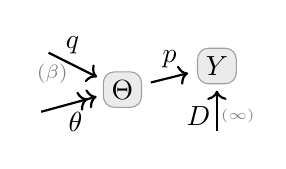
\begin{tikzpicture}[center base]
			\node[dpad0] (theta) at (0,0) {$\Theta$};
            \node[dpad0] (Y) at (1.2,0.3) {$Y$};
			% \node[dpad0, right=0.7 of theta] (Y) {$Y$};
			%
			\draw[arr] (theta) --
	 			% node[above]{$\overset{{\color{gray}(\beta_f)}}f$}
	 			% node[above]{$f^{{\color{gray}(\beta_f)}}$}
	 			node[above]{$p$}
				(Y);
			\draw[arr2, <-] (theta) --
				node[above right=-2pt and -2pt, pos=0.7] {$q$}
				node[below left=-3pt and -4pt,pos=0.6]{{$\color{gray}\scriptstyle(\beta)$}}
				++(-1.0, 0.5);
			% \draw[arr, <-] (theta) --
			% 	node[above right, pos=0.7] {$p^{{\color{gray}(\beta)}}$}
			% 	++(-1.0, 0.4);
			\draw[arr2, <<-] (theta) -- node[below,pos=0.4]{$\theta$} ++(-1.1, -0.3);
			\draw[arr2, <-] (Y) --
                node[left,pos=0.6, inner sep=2pt]{$D$}
                node[right,pos=0.6, inner sep=1pt]
                    {${\color{gray}\scriptscriptstyle(\infty)}$}
                ++(0, -0.9);
		\end{tikzpicture}\!}
		\begin{aligned}
			=\! \Ex_{y \sim D} \log \frac{1}{p(y \,|\,\theta)}
				&+ \beta \log \frac1{q(\theta)} \\[-0.2em]
	            % &\!{\color{gray}- \H(D)}
	            &\!{- \H(D)} %\\[-1em]
		\end{aligned}
		% \beta_f\,
		% \Ex_{y \sim D} \left[\log \frac{1}{f(y \mid \theta_0)} \right]
        %
	\end{equation}
\end{linked}

If our prior is the (discretized) unit gaussian $p(\theta) \!=\! \frac{1}{k} \exp(-\frac12 \theta^2)$ for some constant $k$, then the right hand side of \eqref{eq:regularize} becomes
\[ \underbrace{\Ex\nolimits_{D}\! \left[\log \frac{1}{p(Y \,|\, \theta)} \right]}
	_{\substack{\text{Cross entropy loss}\\(\text{data-fit cost of $\theta$})}}%(f_\theta; D)
	+ \!\!\!\!\!\underbrace{~\frac\beta2 \theta_0^2~}_{\substack{\ell_2 \text{ regularizer}\\(\text{complexity cost of $\theta_0$})}} \!\!\!\!\!
	{\color{gray!80} \underbrace{+ \beta \log k - \H(D)}_{\text{constant in $f, \theta_0$}}}\;, \]
which is the $\ell_2$ regularized version of \cref{prop:expected-surprise}.
Moreover, the regularization strength corresponds exactly to the confidence $\beta$.
What about other priors? It is not difficult to see that if we use a (discretized) centered unit Laplacian prior, $p(\theta) = \frac1k \exp(-|\theta|)$, the second term instead becomes $\beta |\theta_0|$, which is $\ell_1$ regularization.
More generally, to consider any complexity measure $U(\theta)$, we need only include the Gibbs distribution $\Pr_U(\theta) \propto \exp(-U(\theta))$ into our PDG.
%% TODO TOCUT %%%%% True. But helpful??
% And if we lift the requirement that $\theta_0$ be a point mass, the optimal distribution over $\theta$ is the posterior distribution after a Baysian update.
%
We remark that there is nothing special about cross entropy here;
%joe1*: Saying you can do it for one other proposition doesn't seem
%like convincing evidence that it's quite general
%oli1: oops.
% such a prior may be added to the pdg of \cref{prop:MSE} to instead
% regularize square loss. 
% Such a priors may be added to any PDG to effectively add regularization terms.
any of the objectives we describe can be regularized in this way.

\section{VARIATIONAL OBJECTIVES AND BOUNDS}
\label{sec:theory}

\subsection{PDGs and Variational Inference}
\label{sec:variational}

% \todo add the equivalence results between PDGs and VAEs



The fact that the incompatibility of $\dg M$ with a \emph{specific} joint distribution $\mu$ is an upper bound on the inconsistency (i.e., the score of the \emph{best} such joint distribution) is not a deep one (although it does suggest a variational approach to inference in PDGs, which we describe in parallel work).
% but it does yield an efficient approximate inference procedure for PDGs: choose a tractable parametric family $\mathcal P$ of joint distributions $\mu$, and optimize \eqref{eq:semantics}. Making this precise is the focus of a parallel work.
Here, we focus on the more surprising converse:  PDG semantics capture interesting features of variational inference and provides a graphical proof language for it.
%, which can be notoriously difficult to track symbolically.

To demonstrate, we begin by recounting the standard development of the `Evidence Lower BOund' (ELBO), a standard objective for training latent variable models \parencite[\S2.2]{blei2017variational}, and then show that it arises naturally as the inconsistency of the obvious PDG.
Suppose we have a joint distribution $p(X,Z)$, but only have access to observations $X$.
In service of adjusting $p(X,Z)$ to make our observations more likely, we would like to maximize $\log p(X)$, the ``evidence'' of $X$.
Unfortunately, computing $p(X) = \int p(X,z)\, \mathrm d z$ requires integrating over $Z$, which can be intractable.
%
% The variational approach is as follows: fix a family of distributions $\mathcal Q$ that is easy to sample from, choose some $q \in \mathcal Q$, and assume that $Z \sim q$.
% ; to start, we guess $q_0(Z)$.
% Now it's easy to sample $Z$ (by assumption), but $q_0$ is likely to be inconsistent with $p$. But if, while optimizing $p$ to best fit the data, we also optimize $q$ so that it closly mirrors $p$, (and if $\mathcal Q$ is expressive enough), we can avoid computing the ``evidence''  $\log p(x) = \log \int p(x,z)\, \mathrm d z$.
%% For fixed $p$, we are interested in $q^*_p := \argmin_{q \in \mathcal Q} \kldiv{q(Z)}{p(Z\mid x)}$.
% But only by being clever. The straightforward divergence-minimizing approach to both optimization problems (the choice of $p$ and $q$) requires computing this integral \cite[\S2.2]{blei2017variational}. Instead, $q$ and $p$ are chosen so as to maximize
% Now, we can sample $Z$ from $q$, so we can compute 
% $
%     \Ex_{z \sim q} \frac{p(x,z)}{q(z)} =
%     \int_{z} q(z) \frac{p(x,z)}{q(z)} \mathrm dz=
%     \int p(x,z) \mathrm d z = p(z)
% $
The variational approach is as follows: fix a family of distributions $\mathcal Q$ that is easy to sample from, choose some $q(Z) \in \mathcal Q$, and define
$\mathrm{ELBO}_{p,q}(x) := \Ex_{z \sim q} \log \frac{p(x,z)}{q(z)}$.
This is something we can estimate, since we can sample from $q$. By Jensen's inequality, 
\[
    \mathop{\mathrm{ELBO}}\limits_{p,q}(x)
    =\! \Ex_{q} \log \frac{p(x,Z)}{q(Z)}
    % = \int_{z} q(z) \log  \frac{p(x,z)}{q(z)} \mathrm dz 
    \le  \log \Big[\! \Ex_{q}\! \frac{p(x,Z)}{q(Z)} \Big]\!
    = \log p(X).
    % \int p(x,z) \mathrm d z = p(z)
\]
with equality if $q(Z) = p(Z)$. 
So to maximize $p(X)$, it suffices to adjust $p$ and $q$ to maximize $\mathrm{ELBO}_{p,q}(x)$,%
    \footnote{For many iid samples: $\max_{p,q}\sum_{x \in \xsamp}\mathrm{ELBO}_{p,q}(x)$.}
 provided $\mathcal Q$ is expressive enough.
    
% $\mathrm{ELBO}_{p,\xsamp}(q) :=
%     \sum_{x \in \xsamp} \mathrm{ELBO}_{p,q}(x)
% $. 
% where
% \begin{equation}
% 	% \mathrm{ELBO}_{p,\xsamp}(q) :=
% 	%  	\sum_{x \in \xsamp} \mathrm{ELBO}_{p,q}(x)~,
% 	% \qquad \qquad\text{where}
%     %\qquad
% 	\mathrm{ELBO}_{p,q}(x) := \Ex_{z \sim q} \log \frac{p(x,z)}{q(z)}, \label{eq:elbo}
% \end{equation}

% We will now see that this tie extends to latent variable models in a nice way.
The formula for the ELBO is somewhat difficult to make sense of, especially if $p$ and $q$ are densities.%
\footnote{Such expressions }
% (see \cref{remark:continuous}).
% in which case the units don't cancel in the logarithm, making it an ill-defined physical quantity (see \cref{remark:continuous}).
%joe1*: mass functions comes completely out of the blue here.  If you
%mean mass functions as in Demspter-Shafer, then you must explain
%this.  Actually, whatever you mean, you must explain it.  Idon't see
%where this interpretation has any impact on your propositin.
%TODO
Nevertheless, if we interpret $p$ and $q$ are mass functions, it turns
out that the ELBO also arises naturally as the inconsistency of the
appropriate PDG. 

\begin{linked}{prop}{pdg-elbo-x}%[Capturing the ELBO]
		% \label{prop:pdg-elbo-x}
	% If $p(X,Z)$ is a joint probabilistic model of observed variables $X$ and hidden variables $Z$, and $q(Z)$ is any distribution
	% That is,
	The negative ELBO is the inconsistency of the PDG containing $p,q$, and $x$, with very high confidence in $q$.
	That is,
    \vspace{-0.8em}
	\[
	-\mathrm{ELBO}_{p,q}(x) =
		% \lim_{t \to \infty}
	 \aar[\Bigg]{
% 	  \Inc\left(
		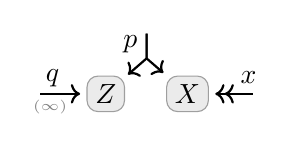
\begin{tikzpicture}[center base]
			\node[dpad0] (Z) {$Z$};
			\node[dpad0,right=.5 of Z] (X) {$X$};
			\coordinate (A) at ($ (X)!.5!(Z) + (0,0.8)$);
			\draw[arr1] (A) -- node[left, inner sep=3pt]{$p$} ++(0,-0.35) -- (X);
			\draw[arr1] (A) -- ++(0,-0.35) -- (Z);
%
			\draw[arr2, <<-] (X) --  node[above,pos=0.8]{$ x$} ++(0.9, 0);
			\draw[arr2, <-] (Z) --
                node[above,pos=0.65, inner sep=2pt]{$q$}
                node[below,pos=0.7, inner sep=2pt]{${\color{gray}\scriptscriptstyle(\infty)}$}
                ++(-0.9, 0);%
			%\scriptstyle q^{\{\beta =\infty\}}
			% \ar[r,"p"] \& Z \ar[r,"p", bend left] \& X \ar[l,"q", bend left] \& \ar[l, two heads, "x"']
		\end{tikzpicture}
		}%_{\!\!0}
% 		\right)
		.
	\]
\end{linked}



%
% The proof of \cref{prop:pdg-elbo-x} %, lke that of \cref{prop:pdg-Ix},
%  hinges critically on the fact that we force a single sample $x$; its PDG does not capture the whole context $\xsamp$.
% Nevertheless, we get an analogous result when we replace the sample $x$ with the entire data distribution $\datadist\xsamp$, which differs only in that the expression is offset by the entropy of the data distribution.
%
%
% \begin{prop}\label{prop:pdg-elbo-X}
% 	Consider a model $p(X,Z)$, auxiliary distribution $q(Z)$, and samples $\xsamp = \{x^{(i)}\}$ defining a data distribution $\datadist\xsamp$.
% 	The following are equal:
% 	\begin{enumerate}[label=(\arabic*)]
% 		\item $- \Ex_{\datadist\xsamp} \mathrm{ELBO}_{p,q}(X)$
% 		\item $\displaystyle\bbr{\,p\,}(q \otimes \datadist\xsamp) + \H(\datadist\xsamp)$
% 		\item \(\displaystyle%\lim_{\beta_q, \beta_{\datadist\xsamp} \to \infty}
% 			% \lim_{t \to \infty}
% 		  \aar[\Bigg]{
% 		  \begin{tikzpicture}[center base]
% 	  		\node[dpad0] (Z) {$Z$};
% 	  		\node[dpad0,right=.5 of Z] (X) {$X$};
% 	  		\coordinate (A) at ($ (X)!.5!(Z) + (0,0.7)$);
% 	  		\draw[arr1] (A) -- node[right]{$ p$} ++(0,-0.25) -- (X);
% 	  		\draw[arr1] (A) -- ++(0,-0.25) -- (Z);
% 	  %
% 	  		\draw[arr1, <-] (X) --  node[above,pos=0.2,anchor=south west]{$ {\datadist\xsamp}!$} ++(0.9, 0);
% 	  			% ^{\{\beta=\beta_0\}}
% 	  		\draw[arr1, <-] (Z) -- node[above]{$ q! $} ++(-0.9, 0);
% 	  	\end{tikzpicture} }_1 + \H(\datadist\xsamp)\)
% 	\end{enumerate}
%
% \end{prop}
% \begin{proof}
%
% \end{proof}



% The use of the ELBO as an objective is often justified by the fact that it is a lower bound on the log likelihood of partial observation $X=x$ (the evidence), which is usually proved with some algebra and Jensen's inequality.
% , or alternatively, but appeal to the non-negativity of relative entropy \cite{elboproofs}.
Owing to its structure, a PDG is often more intuitive and easier to work with than the formula for its inconsistency. 
To illustrate,
we now give a simple and visually intuitive proof of the bound traditionally used to motivate the ELBO, via \cref{lemma!}:
% We now give a very simple diagrammatic proof by via \cref{lemma!}:
$\log \frac1{p(x)} = $
\[
% \log \frac{1}{p(x)} =
	 \aar[\Bigg]{
		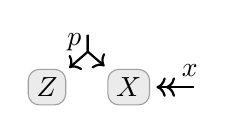
\begin{tikzpicture}[center base]
			\node[dpad0] (Z) {$Z$};
			\node[dpad0,right=.5 of Z] (X) {$X$};
			\coordinate (A) at ($ (X)!.5!(Z) + (0,0.7)$);
			\draw[arr1] (A) -- node[left, inner sep=2pt]{$p$} ++(0,-0.25) -- (X);
			\draw[arr1] (A) -- ++(0,-0.25) -- (Z);
			\draw[arr2, <<-] (X) --  node[above,pos=0.8]{$ x$} ++(0.9, 0);
			% \draw[arr2, <<-] (X) --  node[left,pos=0.8]{$x$} ++(0.2, 0.8);
		\end{tikzpicture}
		}%_{\!\!0}
	\le
    % \lim_{t \to \infty}
	 \aar[\Bigg]{
% 	  \Inc\left(
		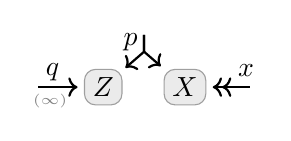
\begin{tikzpicture}[center base]
			\node[dpad0] (Z) {$Z$};
			\node[dpad0,right=.5 of Z] (X) {$X$};
			\coordinate (A) at ($ (X)!.5!(Z) + (0,0.7)$);
            \draw[arr1] (A) -- node[left, inner sep=2pt]{$p$} ++(0,-0.25) -- (X);
			\draw[arr1] (A) -- ++(0,-0.25) -- (Z);
%
			\draw[arr2, <<-] (X) --  node[above,pos=0.8]{$ x$} ++(0.9, 0);
            % \draw[arr2, <<-] (X) --  node[left,pos=0.8]{$x$} ++(0.2, 0.8);
			% \draw[arr2, <-] (Z) -- node[above,pos=0.6]{$ q!$} ++(-0.9, 0);%
			\draw[arr2, <-] (Z) -- node[above, inner sep=2pt,pos=0.6]{$q$}
                node[below, inner sep=2pt, pos=0.65]{\rotatebox{0}{${\color{gray}\scriptscriptstyle(\infty)}$}}
                ++(-0.9, 0.0);
                % ++(-0.3, 0.75);%
			% \ar[r,"p"] \& Z \ar[r,"p", bend left] \& X \ar[l,"q", bend left] \& \ar[l, two heads, "x"']
		\end{tikzpicture}
		}%_{\!\!0}
% 		\right)
    % = \mathop{\mathrm{NELBO}}\limits_{p,q}(x).
\]
$= - \mathrm{ELBO}_{p,q}(x)$.~
The first and last equalities are \Cref{prop:marginal-ll,prop:pdg-elbo-x} respectively.
 % and the inequality is an instance of \Cref{lemma!}.
%% This is fine material, but we don't have space for it...
% We submit that this proof is more intuitve and gives a clearer picture of why it should be true. The second PDG has more edges, so it must be at least as inconsistent.
% Furthermore, this picture shows us that if we simultaneously vary $q(Z)$ within an expressive enough class of distributions, the inequality is also tight, because the distribution that realizes the smallest inconsistency must have some marginal on $Z$ --- and taking $q$ to be that distribution will incur no additional inconsistency.
We submit that our presentation has substantial pedagogical benefits. The second PDG has more edges so it is clearly at least as inconsistent. Furthermore, it's easy to see that equality holds when $q(Z) = p(Z)$: the best distribution for the first PDG has that marginal anyway, so insisting on it incurs no further inconsistency.
% so the constraint is already satisfied.

 % We also have analog analog holds for the entire dataset at once, which is more easily formulated with a slightly different variational form in the next section.

% \begin{align*}
% \ell(p;\xsamp) &=
% 	 \aar[\Bigg]{
% 	 % \Inc\left(
% 		\begin{tikzpicture}[center base]
% 			\node[dpad0] (Z) {$Z$};
% 			\node[dpad0,right=.5 of Z] (X) {$X$};
% 			\coordinate (A) at ($ (X)!.5!(Z) + (0,0.7)$);
% 			\draw[arr1] (A) -- node[right]{$ p$} ++(0,-0.25) -- (X);
% 			\draw[arr1] (A) -- ++(0,-0.25) -- (Z);
% %
% 			\draw[arr1, <<-] (X) --  node[above,pos=0.8]{$ \datadist\xsamp$} ++(0.9, 0);
% 			% \draw[arr1, <-] (Z) -- node[above]{$ q$} ++(-0.9, 0);
% 		\end{tikzpicture}
% 		}%_{\!\!0}
% 		% \right)
% 		 + \H(\datadist\xsamp) \\
% 		&\le
% 			\lim_{t \to \infty}
% 		  \aar[\Bigg]{
% 		  \begin{tikzpicture}[center base]
% 	  		\node[dpad0] (Z) {$Z$};
% 	  		\node[dpad0,right=.5 of Z] (X) {$X$};
% 	  		\coordinate (A) at ($ (X)!.5!(Z) + (0,0.7)$);
% 	  		\draw[arr1] (A) -- node[right]{$ p$} ++(0,-0.25) -- (X);
% 	  		\draw[arr1] (A) -- ++(0,-0.25) -- (Z);
% 	  %
% 	  		\draw[arr1, <-] (X) --  node[above,pos=0.2,anchor=south west]{$ {\datadist\xsamp}^{\{\beta= t\}}$} ++(0.9, 0);
% 	  			% ^{\{\beta=\beta_0\}}
% 	  		\draw[arr1, <-] (Z) -- node[above]{$q^{\{\beta= t\}} $} ++(-0.9, 0);
% 	  	\end{tikzpicture} } + \H(\datadist\xsamp) = - \Ex_{\datadist\xsamp} \mathrm{ELBO}_{p,q}(X),
% \end{align*}
% which holds for the same reason.


\subsection{Variational Auto-Encoders and PDGs}

An autoencoder is a probabilistic model intended to compress a
variable $X$ (e.g., an image) to a compact latent representation
%joe1: another run-on
%$Z$, and its structure is given  by two conditional distributions: 
$Z$. Its structure is given by two conditional distributions:
an encoder $e(Z \mid X)$, and a decoder $d(X \mid Z)$.
Of course, not all pairs of cpds fill this role equally well.
Perhaps most importantly, we would to have low \emph{reconstruction error} \eqref{eq:rec}---when we decode an encoded image, we would like it to be reasonably similar to the original.
\vspace{-0.5em}
\begin{equation}
 \mathrm{Rec}(x) := \!\! \Ex_{z \sim e \mid x} \, \underbrace{\,\mathrm I_{d\mid z}(x)~\vphantom{\bigg|}}_{\mathclap{\left(\;\substack{\text{additional bits required to}\\\text{decode $x$ from $z$, its encoding}}\;\right)}}
	\!= \sum_z e(z \,|\, x) \log \frac1{d(x \,|\, z)}\label{eq:rec}
\end{equation}

% It just so happens that $\mathrm{Rec}(x) =
% \aar*{\begin{tikzpicture}[center base]
%     \node[dpad0] (Z) {$Z$};
%     \node[dpad0,right=.6 of Z] (X) {$X$};
%     \draw[arr2, ->] (X) to[bend left=60]
%         node[below, inner sep=2pt]{$e$}
%         node[above, inner sep=2pt]{${\color{gray}\scriptscriptstyle(\infty)}$} (Z);
%     \draw[arr2, ->] (Z) to[bend left=50]
%         node[above, inner sep=2pt]{$d$} (X);
%     \draw[arr2, <<-] (X) --
%         node[above,pos=0.8]{$x$}
%         ++(0.9, 0);
% \end{tikzpicture}}$.
% Note the similarity to the cross entropy objective from before, except in place of our

There are other desiderata as well. It would be nice if the
distribution on $Z$ had a nice form---perhaps factoring into
independent features, which we might use to describe $X$. We encode
%joe1*: I don't see how beliefs can encode wishes at all. Wishes are
%captured by utilities, not probabilities.  I'm lost.
%oli1: the whole point is that probabilities/objectives 
% are a blurred line. I'll tweak the wording a little.
% this wish in the form of a belief $p(Z)$, known as a variational
this wishful thinking as a belief $p(Z)$, known as a variational
prior. 

The data of a \emph{variational} auto-encoder
\parencite{kingma2013autoencoding}
consists of $e(Z|X)$, $d(X|Z)$, and $p(Z)$.
The encoder $e(Z|X)$ can be used as a variational approximation of $Z$, differing from $q(Z)$ of \Cref{sec:variational} only in that it can depend on $X$. Here, the analogue of the ELBO becomes
\vspace{-0.5em}
\begin{align*}
	\mathrm{ELBO}_{p,e,d}(x) &= \Ex_{z \sim e|x} \left[\log \frac{p(z) d(x\mid z)}{e(z\mid x)} \right] \\
		% &= \Ex_{z \sim e|x}\left[ \log \frac{p(z)}{e(z\mid x)}  \right] - \Ex_{z \sim e|x} \log \frac1{d(x\mid z)} \\
		&= \kldiv{e(Z|x)}{p} - \mathrm{Rec}(x).
\end{align*}

This gives us the following analog of \cref{prop:pdg-elbo-x}.

\begin{linked}{prop}{pdg-elbo-vae}
	The VaE objective for a sample $x$%
        \dfootnote{See appendix for a multi-sample analog.}
    is the inconsistency of the PDG containing the encoder $e$ (with high confidence, as it defines the encoding), decoder $d$ prior $p$, and $x$.
	That is,
    % \vspace{-1.8em}
    \vspace{-1em}
	\[
	-\mathrm{ELBO}_{p,e,d}(x) =
	 \aar*{
		% \begin{tikzcd}[AmpRep,row sep=1em,column sep=1.5em]
		% 	\ar[r,"p"] \& Z \ar[r,"d", bend left] \& X \ar[l,"e!", bend left] \& \ar[l, two heads, "x"']
		% \end{tikzcd}
		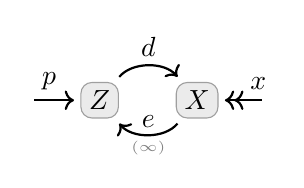
\begin{tikzpicture}[center base]
			\node[dpad0] (Z) {$Z$};
			\node[dpad0,right=.7 of Z] (X) {$X$};
			\draw[arr2, ->] (X) to[bend left=50]
				node[above, inner sep=2pt]{$e$} 
				node[below, inner sep=2pt]{${\color{gray}\scriptscriptstyle(\infty)}$} 
                (Z);
			\draw[arr2, ->] (Z) to[bend left=50]
				node[above]{$ d$} (X);
			\draw[arr2, <<-] (X) --
			  	node[above,pos=0.8]{$ x$}
			 	++(0.9, 0);
			\draw[arr2, <-] (Z) --
				node[above,pos=0.6]{$ p$}
				++(-0.9, 0);%
		\end{tikzpicture}}.
 	\]
    \vspace{-2em}
\end{linked}


\subsubsection{Intuitive Proofs of Variational Bounds}
\Cref{prop:pdg-elbo-vae,prop:pdg-elbo-vae-whole} can be used to derive the variational lower bound. Once again, the addition of the edge $e$ cannot decrease the inconsistency (\cref{lemma!}), but believing it with high confidence does make it possible to generate the encoding for a sample, making inference tractable.
This result in the following simple visual proof:
%joe1: the layout here needs to be improved
%TODO
~~$- \log \Pr(x) =$
\vspace{-1.4em}
\[
	\aar[\bigg]{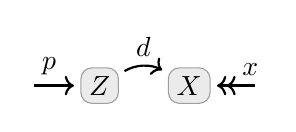
\begin{tikzpicture}[baseline=-0.5ex]
	   \node[dpad0] (Z) {$Z$};
	   \node[dpad0,right=.6 of Z] (X) {$X$};
	   \draw[arr2, ->] (Z) to[bend left=30]
		   node[above]{$ d$} (X);
	   \draw[arr2, <<-] (X) --
		   node[above,pos=0.8]{$ x$}
		   ++(0.9, 0);
	   \draw[arr2, <-] (Z) --
		   node[above,pos=0.6]{$ p$}
		   ++(-0.9, 0);%
	\end{tikzpicture}}
 	\le
 	\aar*{
   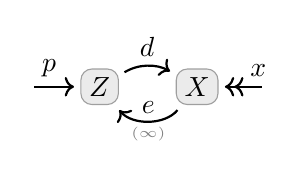
\begin{tikzpicture}[center base]
       \node[dpad0] (Z) {$Z$};
       \node[dpad0,right=.7 of Z] (X) {$X$};
       \draw[arr2, ->] (X) to[bend left=50]
           node[above, inner sep=2pt]{$e$} 
           node[below, inner sep=2pt]{${\color{gray}\scriptscriptstyle(\infty)}$} 
           (Z);
       \draw[arr2, ->] (Z) to[bend left=30]
           node[above]{$ d$} (X);
       \draw[arr2, <<-] (X) --
           node[above,pos=0.8]{$ x$}
           ++(0.9, 0);
       \draw[arr2, <-] (Z) --
           node[above,pos=0.6]{$ p$}
           ++(-0.9, 0);%
   \end{tikzpicture}}
\]
\vskip-1.2em
$= -\mathrm{ELBO}_{p,e,d}(x).$
Here $\Pr(X)$ is the marginal of $p(Z)d(X \mid Z)$ on $X$.
In the appendix, we also give the analogue for many samples, with a single application of the inequality.

\subsection{\texorpdfstring{$\beta$}{beta}-VaE Objective}

The ELBO is not the only objective that has been used to train networks with the a VaE structure.
In the most common variant, 
% Higgins et. al. 
% \cite{higgins2016beta}
\textcite{higgins2016beta}
have argued that the one might want to weight the reconstruction error \eqref{eq:rec} and KL term differently.  They suggest an objective of the form
\vskip-1.2em
\[ \beta\text{-}\mathrm{ELBO}_{p,e,d}(x) := \mathrm{Rec}(x) - \beta \kldiv{e(Z|x)}{p}\]
\vskip-0.5em
which for $\beta = 1$ is equivalent to the ELBO as before. The authors view it as a regularization parameter, annd argue that in some cases, you can do better with a stronger prior.
%joe1
%Sure enough, the $\beta$-VaE objective is the inconsistency of same
Sure enough, the $\beta$-VaE objective is the inconsistency of the same
%joe1
%PDG as before, but with confidence $\beta$ in $p(Z)$.\footnote{the two
PDG as before, but with confidence $\beta$ in $p(Z)$.\footnote{The two
parameters even share a name, both coming from thermodynamic $\beta$
(inverse temperature).} 


\section{FREE ENERGY AND INCONSISTENCY}
% The factors of a factor graph, which in isolation indicate relative probabilities.
The weighted factor graph (WFG) $\Psi = (\phi_j, \theta_j)_{j \in \cal J}$, where each $\theta_j$ is a real weight, $j$ is associated with a subset of variables $\mathbf X_j$, and  $\phi_j : \mathbf X_j \to \mathbb R$ determines a distribution by
\vskip-1.2em
\[ \Pr\nolimits_\Psi(\mat x) \propto \prod_{j \in J} \phi_j(\mat x_j)^{\theta_j} \]
\vskip-0.7em
The normalization constant $Z_{\Psi}$, is given by
% \begin{equation*}
\(
	Z_{\Psi} := \sum_{\mat w} \prod_{j \in \mathcal J} \phi_j(\mat w_j)^{\theta_j},
\)
% \end{equation*}
%joe1: I can't parse the rest of this sentence
% TODO
and is known as the \emph{partition function}, and is computing it is
intimately related to many probabilistic inference tasks. 

If every factor is a cpd, and every variable is the target of at least one edge, then $Z_\Psi$ is at most 1, so $-\log Z_\Psi$ is non-negative, and measures how far away the product of factors is from being normalized. Thus, it is in some sense a measure of inconsistency of a factor graph.
It turns out that this intuition coincides with our notion of PDG 1-inconsistency. 

\begin{linked}{prop}{fg-inconsistency-is-partition-function}
	For any weighted factor graph
	$\Psi$, we have $\aar{\PDGof{\Psi}}_1 = - \log Z_{\Psi}$.
\end{linked}

Outside of computer science, such factored exponential families form
%joe1: another run-on sentence
%the mathematical backbone of statistical mechanics, and in this world
the mathematical backbone of statistical mechanics. In this setting,
$- \log Z_{\Psi}$ is the Heimholtz free energy. The principle of
free-energy minimization has been enormously succesful in describing
the evolution of chemical systems. 
%TODO: CITATIONS
% Many thermodynamic quantities
% (e.g., as internal energy, free energy, pressure, volume, and entropy) can
% be obtained by taking various partial derivatives of $Z_\Psi$, and calculating the partition function is closely related to infering marginal distributions \cite{}.

\section{FINAL REMARKS}

% DISCUSSION GOES HERE.

We have now seen that PDG semantics not only capture structured objects such as Bayesian Networks and Factor Graphs as in \textcite{richardson2020probabilistic}, but in the same stroke also generate many standard loss functions, including some non-trivial ones as a simple consequence of carefully articulating modeling assumptions.
Viewing loss functions in this way also has beneficial side effects, including an intuitive visual proof language for reasoning about the relationships between them.

%joe1*: I *strongly* suggest removing this paragraph.   You have
%provided no evidence whatsoever that what you are doing is in the
%spirit of cognitive dissonance (which is about how an agent handles
%conflicting beliefs, largely by ignoring upsetting information).  
% Taking a step back, we submit that this approach to modeling agents, which is similar in spirit to the theory of \emph{cognitive dissonance} \cite{}, is also more plausible for humans than one that supposes we minimize expectations of some concrete, exogenously given measure of (dis)utility.
% We also believe that our ``universal loss function'' will be of substantial interest to the AI safety community.
 % blurring the line between model and objective.

\subsubsection*{Acknowledgements}
% All acknowledgments go at the end of the paper, including thanks to reviewers who gave useful comments, to colleagues who contributed to the ideas, and to funding agencies and corporate sponsors that provided financial support.
% To preserve the anonymity, please include acknowledgments \emph{only} in the camera-ready papers.


% \subsubsection*{References}
%joe1: lotys of problems here:
%- [8] and [9] are the same, mwention Mackay twice, should have eriods
%afer J and C (this problem also occurs in [4] amd [6]), and the book
%title shoudl be in all caps
%-  In [11], l2 should be L2 ({L}2) in latex
% in [14], Kullback-Leibler should capitalized
%- in [15], Laplace and the journal title shoudl be capitalized

% References follow the acknowledgements.  Use an unnumbered third level
% heading for the references section.  Please use the same font
% size for references as for the body of the paper---remember that
% references do not count against your page length total.

% \bibliographystyle{plain}
% \bibliography{refs}
{
% \raggedright
\printbibliography
}

\clearpage
\onecolumn
\appendix

\section{More Detailed Results}
\subsection{More General Characterizations of Gaussian Predictors}
But before we get there, we first prove a more general result, which is most clearly articulated in terms of a power mean.

\begin{defn}%[power mean]
	The weighted power mean $\mathrm M^w_p(\mathbf r)$ of the collection of real numbers $\mathbf r = r_1, \ldots, r_n$ with respect to the convex weights $w = w_1, \ldots, w_n$ satisfying $\sum_iw_i = 1$, is given by
	\[ \mathrm M^w_p(\mathbf r) := \Big(\sum_{i=1}^n w_i (r_i)^p \Big)^{\frac1p}.\]
	We omit the superscript as a shorthand for the uniform weighting $w_i = \nicefrac{1}{N}$.
	Most standard means, such as those in \cref{tab:power-means}, are special cases.
\end{defn}

\begin{table}
\centering
\renewcommand{\arraystretch}{1.5} % General space between rows (1 standard)
\begin{tabular}{rcl}
	\textbf{Name} & $p$ & \textbf{Formula}\\\hline
	Harmonic&$(p=-1)$:& $\mathrm{HM}_w(\mathbf r) = \faktor1{\left(\sum_{i=1}^n \nicefrac{w_i}{r_i}\right)}$ \\
	Geometric&$(\lim {p\to 0})$:& $\mathrm{GM}_w(\mathbf r) = \prod_{i=1}^n r_i^{w_i}$ \\
	Arithmetic&$(p=1)$:& $\mathrm{AM}_w(\mathbf r) = \sum_{i=1}^n w_i r_i$ \\
	Quadratic&$(p=2)$:& $\mathrm{QM}_w(\mathbf r) = \sqrt{\textstyle\sum_{i=1}^n w_i r_i^2}$\\\hline
	\end{tabular}
	\caption{special cases of the $p$-power mean $\mathrm M_p^w(\mathbf r)$}
	\label{tab:power-means}
\end{table}
% \begin{align*}
% 	\text{Harmonic}~(p=-1):&\quad \mathrm{HM}_w(\mathbf r) = \frac1{\sum_{i=1}^n \nicefrac{w_i}{r_i}} \\
% 	\text{Geometric}~(\lim {p\to 0}):&\quad \mathrm{GM}_w(\mathbf r) = \prod_{i=1}^n r_i^{(w_i)} \\
% 	\text{Arithmetic}~(p=1):&\quad \mathrm{AM}_w(\mathbf r) = \sum_{i=1}^n w_i r_i \\
% 	\text{Quadratic}~(p=2):&\quad \mathrm{QM}_w(\mathbf r) = \sqrt{\textstyle\sum_{i=1}^n w_i r_i^2}.
% \end{align*}

It is well known that $\mathrm M_p^w(\mathbf r)$ is increasing in $p$, and strictly so if not all elements of $\mathbf r$ are identical. In particular, $\mathrm{QM}_w(a,b) > \mathrm{GM}_w(a,b)$ for all $a \ne b$ and positive weights $w$. We now present the result.


\begin{linked}{prop}{inc-two-gaussians}
	Consider a PDG containing two (distinct) conditional Gaussian distributions on a variable $Y$, whose parameters can both depend on a variable $X$. Its inconsistency takes the form
	\begin{align*}
		\aar**{\!\!\!\!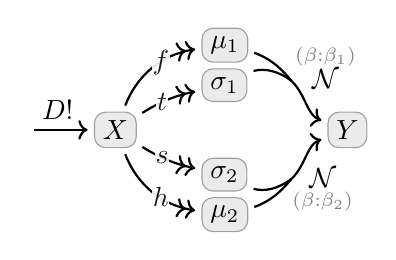
\begin{tikzpicture}[center base]
			\node[dpad0] (Y) {$Y$};
			\node[dpad0,left=2.4 of Y] (X) {$X$};
			\node[dpad0,above right=0.6 and 0.8 of X] (mf) {$\mu_1$};
			\node[dpad0,below right=0.6 and 0.8 of X] (mh) {$\mu_2$};
			\node[dpad0,above right=0.1 and 0.8 of X] (sf) {$\sigma_1$};
			\node[dpad0,below right=0.1 and 0.8 of X] (sh) {$\sigma_2$};
			%
			\draw[arr2, ->>] (X) to[bend left=30]
				node[pos=0.6, inner sep=0.2pt, fill=white, fill opacity=0.9] {$f$} (mf);
				\draw[arr2, ->>] (X) to[bend left=10]
					node[pos=0.4, inner sep=0.2pt, fill=white, fill opacity=0.9] {$t$} (sf);
			\draw[arr2, ->>] (X) to[bend right=30]
					node[pos=0.6, inner sep=0.2pt, fill=white, fill opacity=0.9] {$h$} (mh);
				\draw[arr2, ->>] (X) to[bend right=10]
					node[pos=0.4, inner sep=0.2pt, fill=white, fill opacity=0.9] {$s$} (sh);
			%
			\draw[arr2, <-] (X) to node[pos=0.55, above]{$D!$} +(-1.1, 0);
			\coordinate (C1) at ($(mf)!.5!(sf) + (0.85,-0.2)$);
			\coordinate (C2) at ($(mh)!.5!(sh) + (0.85,+0.2)$);
			% \coordinate (C2) at ($ (X)!.5!(Y) + (0,0.8)$);
			\draw[arr2, ->] (mh) to[bend right=15] (C2) to[out=45,in=-160]
				node[pos=0.25, below right, inner sep=0] {\!\!$\underset{{\color{gray}(\beta:\beta_2)}}{\mathcal N}$} (Y);
			\draw[arr2, -,shorten >=0pt] (sh) to[bend right=25] (C2);
			%
			\draw[arr2, ->] (mf) to[bend left=15] (C1) to[out=-45,in=160]
				node[pos=0.25, above right, inner sep=1pt] {\!\!$\overset{{\color{gray}(\beta:\beta_1)}}{\mathcal N}$} (Y);
			\draw[arr2, -,shorten >=0pt] (sf) to[bend left=25] (C1);
			% \draw (current bounding box.north east) rectangle (current bounding box.south west);
		\end{tikzpicture}\!} %\hspace{-2cm}&\\
		 \! &=
		  	\frac12
			\Ex\nolimits_D \!\!\left[
		 	{\mathrm {HM}}(\beta_1, \beta_2)
				\frac12
			\left( \frac{\mu_1 - \mu_2}
		 		{\mathrm {QM}_{\hat\beta}(\sigma_1,\sigma_2)} \right)^{\!\!2}
			+ {\mathrm {AM}}(\beta_1, \beta_2) \log
				\frac
				{\mathrm {QM}_{\hat\beta}(\sigma_1,\sigma_2)}
				{\mathrm {GM}_{\hat\beta}(\sigma_1,\sigma_2)}
		 \right] \numberthis\label{eq:2gaussians} \\
		 &\color{gray}\hspace{-2cm}= \Ex_{x \sim D} \left[
		 	\frac{\beta_1 \beta_2}2
		 	\frac{\Big(f(x) - h(x)\Big)^2}
		 		% {\mathrm {QM}_{\hat\beta}(s(x),t(x))}
		 		{\beta_2 s(x)^2 + \beta_1 t(x)^2}
			+ \frac{\beta_1 + \beta_2}{2} \log
				\frac
				{\beta_2 s(x)^2 + \beta_1 t(x)^2}
				{(\beta_1 + \beta_2)( s(x)^{\beta_2} t(x)^{\beta_1})^{\frac1{\beta_1+\beta_2}}}
				% {\mathrm {QM}_{\hat\beta}(s(x),t(x))}
				% {\mathrm {GM}_{\hat\beta}(s(x),t(x))}
		 \right]
	\end{align*}
	where  $\hat\beta = (\frac{\beta_2}{\beta_1+\beta_2}, \frac{\beta_1}{\beta_1+\beta_2})$ represents the normalized and reversed vector of conficences $\beta = (\beta_1, \beta_2)$ for the two distributions, and $\mu_1 = f(X)$, $\mu_2 = g(X)$, $\sigma_1 = s(X)$, $\sigma_2 = t(X)$ are random variables over $X$.
\end{linked}




Plugging in $s(x) = t(x) = 1$ and $\beta_1 = \beta_2 = 1$ proves:%\Cref{prop:MSE}:

\recall{prop:MSE}

The equality of the two PDG inconsistencies illustrates an orthogonal point: that PDGs handle composition of functions as one would expect, so that it is equivalent to model an entire process as a single arrow, or to break it into stages, ascribing an arrow to each stage, with one step of randomization.

\subsection{Visual Multi-sample Variational Bound}
\Cref{prop:expected-surprise,prop:pdg-elbo-vae-whole} lets us do the same thing for many i.i.d. datapoints at once, with only a single application of the inequality:
\begin{align*}
	- \log \Pr(\xsamp) = - \log \prod_{i=1}^m \left(\Pr(x^{(i)})\right) =
	- \frac1{m}\sum_{i = 1}^m \log \Pr(x^{(i)})   = &\\
	\H(\datadist\xsamp) + \aar*{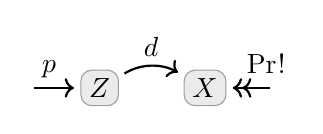
\begin{tikzpicture}[center base]
	   \node[dpad0] (Z) {$Z$};
	   \node[dpad0,right=0.8 of Z] (X) {$X$};
	   \draw[arr2, ->] (Z) to[bend left=30]
		   node[above]{$d$} (X);
	   \draw[arr2, <<-] (X) --
		   node[above,pos=0.8]{$\datadist\xsamp!$}
		   ++(0.9, 0);
	   \draw[arr2, <-] (Z) --
		   node[above,pos=0.6]{$p$}
		   ++(-0.9, 0);%
	\end{tikzpicture}}
 	&\le
 	\aar*{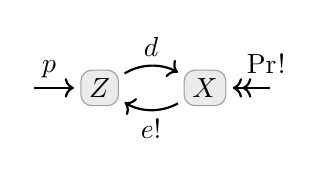
\begin{tikzpicture}[center base]
		\node[dpad0] (Z) {$Z$};
		\node[dpad0,right=.8 of Z] (X) {$X$};
		\draw[arr2, ->] (X) to[bend left=30]
			node[below]{$e!$} (Z);
		\draw[arr2, ->] (Z) to[bend left=30]
			node[above]{$d$} (X);
		\draw[arr2, <<-] (X) --
			node[above,pos=0.8]{$\datadist\xsamp!$}
			++(0.9, 0);
		\draw[arr2, <-] (Z) --
			node[above,pos=0.6]{$ p$}
			++(-0.9, 0);%
	\end{tikzpicture}} + \H(\datadist\xsamp) \\
	&\qquad\qquad= -\Ex_{\datadist\xsamp}\mathop{\mathrm{ELBO}}\limits_{p,e,d}(X)
\end{align*}


\section{Proofs}
\recall{prop:pdg-Ix}
% \csname prop:pdg-Ix\endcsname*
\begin{lproof}\label{proof:pdg-Ix}
	Any distribution $\mu(X)$ that places mass on some $x' \ne x$ will have infinite KL divergence from the point mass on $x$. Thus, the only possibility for a finite consistency arises when $\mu = \delta_x$, and so
	\begin{equation*}
		\aar[\Big] {
		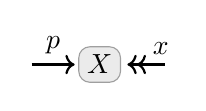
\begin{tikzpicture}[center base]
			\node[dpad0] (X) {$X$};
			\coordinate (A) at ($(X) + (-0.9,0)$);
			\draw[arr1] (A) -- node[above]{$ p$}  (X);
	%
			\draw[arr2, <<-] (X) --  node[above,pos=0.8]{$ x$} ++(0.9, 0);
		\end{tikzpicture}
		}
		= \bbr*{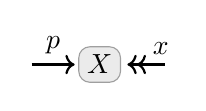
\begin{tikzpicture}[center base]
			\node[dpad0] (X) {$X$};
			\coordinate (A) at ($(X) + (-0.9,0)$);
			\draw[arr1] (A) -- node[above]{$ p$}  (X);
	%
			\draw[arr2, <<-] (X) --  node[above,pos=0.8]{$ x$} ++(0.9, 0);
		\end{tikzpicture}}( \delta_x )
		= \kldiv{\delta_x}{p} = \log \frac{1}{p(x)} = \I_p(x).
	\end{equation*}
\end{lproof}


\begin{linked}{prop}{many-equal-simple}
	Given a model determining a probability distribution with mass function $p(X)$, and samples $\xsamp = \{ x_i \}_{i=1}^m$ determining an empirical distribution $\datadist\xsamp$,  the following are equal, for all $\gamma \ge 0$:
	\begin{enumerate}
	\item The average negative log likelihood $\ell(p; \xsamp) = - \frac{1}{m} \sum_{i=1}^m \log p(x_i)$
	\item The cross entropy of $p$ relative to $\datadist\xsamp$
	\item $\bbr{\,p\,}_\gamma(\datadist\xsamp) ~{\color{gray}~+ (1+\gamma)\H(\datadist\xsamp)}$ \\[-1.4em]
	% FALSE! \item $\bbr{\,p^{\{\alpha=1\}} \,}_1 (\datadist\xsamp^{\{\alpha=1\}})$
	\item \(\aar[\Big] {
		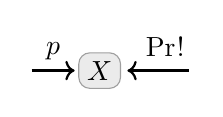
\begin{tikzpicture}[center base]
			\node[dpad0] (X) {$X$};
			\coordinate (A) at ($(X) + (-0.9,0)$);
			\draw[arr1] (A) -- node[above]{$p$}  (X);
			\draw[arr2, <-] (X) --  node[above,pos=0.6]{${\datadist\xsamp}!$} ++(1.2, 0);
				%\overset{\{\beta = \infty\}}
		\end{tikzpicture}
		}_\gamma
		~{\color{gray}~+ (1+\gamma) \H(\datadist\xsamp)}
		\)
	% \item
	% \(\aar[\Bigg] {
	% 	\begin{tikzpicture}[center base]
	% 		\node[dpad0] (X) {$X$};
	% 		\coordinate (A) at ($(X) + (-1.2,0)$);
	% 		\draw[arr1] (A) -- node[above,pos=0.4]{$ \overset {\{\alpha = 1\}} p$}  (X);
	% %
	% 		\draw[arr2, <-] (X) --  node[above,pos=0.6]{$ \overset{\{\beta = \infty,\alpha=\gamma\}}{\datadist\xsamp}$} ++(1.5, 0);
	% 	\end{tikzpicture}
	% 	}\!\bigg._1 \)
\end{enumerate}
\end{linked}
% \recall{prop:many-equal-simple}
\begin{lproof} \label{proof:many-equal-simple}
	The equality of 1 and 2 is standard. The equality of 3 and 4 can be seen by the fact that in the limit of infinite confidence on $\datadist\xsamp$, the optimal distribution must also equal $\datadist\xsamp$, so the least inconsistency is attained at this value.
	Finally it remains to show that the first two and last two are equal:
	\begin{align*}
		\bbr{\,p\,}_\gamma(\datadist\xsamp) + (1+\gamma)\H(\datadist\xsamp)
		&=  \kldiv{\datadist\xsamp}{p} - \gamma \H(\datadist\xsamp)+ (1+\gamma)\H(\datadist\xsamp) \\
		&= \kldiv{\datadist\xsamp}{p} + \H(\datadist\xsamp) \\
		&= \Ex\nolimits_{\datadist\xsamp}\left[\log\frac{\datadist\xsamp}{p} +  \log\frac{1}{\datadist\xsamp}\right]
		= \Ex\nolimits_{\datadist\xsamp}\left[\log\frac{1}{p}\right],
	\end{align*}
	which is the cross entropy, as desired.
\end{lproof}


\recall{prop:marginal-ll}
\begin{lproof}\label{proof:marginal-ll}
	As before, all mass of $\mu$ must be on $x$ for it to have a finite score.
	Thus it suffices to consider joint distributions of the form $\mu(X,Z) = \delta_x(X) \mu(Z)$.
	We have
	\begin{align*}
	\aar*{
		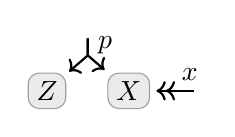
\begin{tikzpicture}[center base]
			\node[dpad0] (Z) {$Z$};
			\node[dpad0,right=.5 of Z] (X) {$X$};
			\coordinate (A) at ($ (X)!.5!(Z) + (0,0.7)$);
			\draw[arr1] (A) -- node[right]{$ p$} ++(0,-0.25) -- (X);
			\draw[arr1] (A) -- ++(0,-0.25) -- (Z);
			\draw[arr2, <<-] (X) --  node[above,pos=0.8]{$ x$} ++(0.9, 0);
		\end{tikzpicture}}
			&= \inf_{\mu(Z)} \bbr*{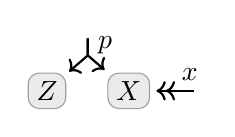
\begin{tikzpicture}[center base]
				\node[dpad0] (Z) {$Z$};
				\node[dpad0,right=.5 of Z] (X) {$X$};
				\coordinate (A) at ($ (X)!.5!(Z) + (0,0.7)$);
				\draw[arr1] (A) -- node[right]{$ p$} ++(0,-0.25) -- (X);
				\draw[arr1] (A) -- ++(0,-0.25) -- (Z);
				\draw[arr2, <<-] (X) --  node[above,pos=0.8]{$ x$} ++(0.9, 0);
			\end{tikzpicture}}\Big(\delta_x(X)\mu(Z)\Big)  \\
			&= \inf_{\mu(Z)}\kldiv[\Big]{\delta_x(X)\mu(Z)}{p(X,Z)} \\
			&= \inf_{\mu(Z)}\Ex_{z \sim \mu} \log \frac{\mu(z)}{p(x,z)}
			~= \inf_{\mu(Z)}\Ex_{z \sim \mu} \log \frac{\mu(z)}{p(x,z)}\frac{p(x)}{p(x)} \\
			&= \inf_{\mu(Z)}\Ex_{z \sim \mu} \left[ \log \frac{\mu(z)}{p(z \mid x)} + \log \frac{1}{p(x)} \right] \\
			&= \inf_{\mu(Z)} \Big[\kldiv{\mu(Z)}{p(Z\mid x)}\Big] + \log \frac{1}{p(x)} \\
			&= \log \frac{1}{p(x)} = \I_p(x) & \text{[Gibbs Inequality]}
	\end{align*}
\end{lproof}


\begin{linked}{prop}{pdg-loglikelihood}
	The average negative log likelihood $\ell(p;x) := -\frac{1}{|\xsamp|}\sum_{x \in \xsamp} \log p(x)$ (which is also the cross entropy) is the inconsistency of the PDG containing $p$ and the data distribution $\datadist\xsamp$, plus the entropy of the data distribution (which is constant in $p$).
	That is,
	\[
	\ell(p;\xsamp) =
	 \aar[\Bigg]{
	 % \Inc\left(
		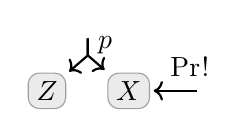
\begin{tikzpicture}[center base]
			\node[dpad0] (Z) {$Z$};
			\node[dpad0,right=.5 of Z] (X) {$X$};
			\coordinate (A) at ($ (X)!.5!(Z) + (0,0.7)$);
			\draw[arr1] (A) -- node[right]{$p$} ++(0,-0.25) -- (X);
			\draw[arr1] (A) -- ++(0,-0.25) -- (Z);
			%
			\draw[arr1, <-] (X) --  node[above,pos=0.8]{$\datadist\xsamp!$} ++(0.9, 0);
			% \draw[arr1, <-] (Z) -- node[above]{$ q$} ++(-0.9, 0);
		\end{tikzpicture}
		}%_{\!\!0}
		% \right)
		+ \H(\datadist\xsamp).
	\]
\end{linked}
% \recall{prop:pdg-loglikelihood}
% 
\begin{lproof}\label{proof:pdg-loglikelihood}
	The same idea as in \cref{prop:marginal-ll}, but a little more complicated.

	\begin{align*}
	\aar*{
		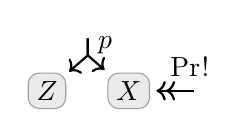
\begin{tikzpicture}[center base]
			\node[dpad0] (Z) {$Z$};
			\node[dpad0,right=.5 of Z] (X) {$X$};
			\coordinate (A) at ($ (X)!.5!(Z) + (0,0.7)$);
			\draw[arr1] (A) -- node[right]{$p$} ++(0,-0.25) -- (X);
			\draw[arr1] (A) -- ++(0,-0.25) -- (Z);
			\draw[arr2, <<-] (X) --  node[above,pos=0.8]{$\datadist\xsamp!$} ++(0.9, 0);
		\end{tikzpicture}}
			&= \inf_{\mu(Z \mid X)} \bbr*{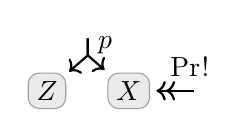
\begin{tikzpicture}[center base]
				\node[dpad0] (Z) {$Z$};
				\node[dpad0,right=.5 of Z] (X) {$X$};
				\coordinate (A) at ($ (X)!.5!(Z) + (0,0.7)$);
				\draw[arr1] (A) -- node[right]{$ p$} ++(0,-0.25) -- (X);
				\draw[arr1] (A) -- ++(0,-0.25) -- (Z);
				\draw[arr2, <<-] (X) --  node[above,pos=0.8]{$ \datadist\xsamp!$} ++(0.9, 0);
			\end{tikzpicture}}\Big(\datadist\xsamp(X) \mu(Z \mid X)\Big)  \\
			&= \inf_{\mu(Z \mid X)}\kldiv[\Big]{\datadist\xsamp(X) \mu(Z \mid X)}{p(X,Z)} \\
			&= \inf_{\mu(Z \mid X)}
				\Ex_{\substack{x \sim \datadist\xsamp \\ z \sim \mu}}
					\log \frac{\mu(z \mid x)\datadist\xsamp(x)}{p(x,z)} \\
			&= \frac{1}{|\xsamp|}\inf_{\mu(Z\mid X)}\sum_{x \in \xsamp}
				\Ex_{z \sim \mu(Z\mid x)} \log \frac{\mu(z \mid x) \datadist\xsamp(x) }{p(x,z)}\frac{p(x)}{p(x)} \\
			&= \frac{1}{|\xsamp|}\inf_{\mu(Z \mid X)}\sum_{x \in \xsamp}\Ex_{z \sim \mu} \left[ \log \frac{\mu(z)}{p(z \mid x)} + \log \frac{1}{p(x)} - \log \frac{1}{\datadist\xsamp(x)} \right] \\
			&= \frac{1}{|\xsamp|}\sum_{x \in \xsamp} \left[
				\inf_{\mu(Z)} \Big[\kldiv{\mu(Z)}{p(Z\mid x)}\Big] + \log \frac{1}{p(x)} \right] - \H(\datadist\xsamp) \\
			&= \frac{1}{|\xsamp|}\sum_{x \in \xsamp} \log \frac{1}{p(x)} - \H(\datadist\xsamp)
			= \frac{1}{|\xsamp|} \sum_{x \in \xsamp} I_p(x) - \H(\datadist\xsamp) \\
			\Big(\quad&= \kldiv{\datadist\xsamp}{p(X)} \quad \Big)
	\end{align*}
\end{lproof}


\recall{prop:supervised-cross-entropy}
\begin{lproof} \label{proof:supervised-cross-entropy}
	$\datadist\xysamp$ has high confidence, it is the only joint distribution $\mu$ with finite score. Since $f$ is the only other edge, the inconsistency is therefore
	\begin{align*}
	\Ex_{x \sim \datadist\xysamp} \kldiv[\Big]{\datadist\xysamp(Y\mid x)}{f(Y\mid x)}
		&= \Ex_{x,y \sim \datadist\xysamp} \left[\log \frac{\datadist\xysamp(y\mid x)}{f(y\mid x)}\right]\\
		&= \Ex_{x,y \sim \datadist\xysamp} \left[ \log \frac{1}{f(y\mid x)} - \log \frac{1}{\datadist\xysamp(y\mid x)} \right] \\
		&= \frac1{|\xysamp|}\sum_{(x,y) \in \xysamp} \left[\log \frac1{f(y \mid x)}\right] \quad - \H_{\datadist\xysamp}(Y\mid X)
	\end{align*}
	\[  \]
\end{lproof}

\recall{prop:accuracy}
\begin{lproof}\label{proof:accuracy}
	Becuase $f$ is deterministic, for every $x$ in the support of a joint distribution $\mu$ with finite score, we must have $\mu(Y\mid x) = \delta_f$, since if $\mu$ were to place any non-zero mass $\mu(x,y) = \epsilon > 0$  on a pont $(x,y)$ with $y \ne f(x)$ results in an infinite contribution to the KL divergence
	\[ \kldiv{\mu(Y\mid x)}{\delta_{f(x)}} =
	 	\Ex_{x,y \sim \mu} \log \frac{\mu(y\mid x)}{\delta_{f(x)}} \ge \mu(y,x) \log \frac{\mu(x,y)}{\mu(x) \cdot \delta_{f(x)}(y)} =  \epsilon \log \frac{\epsilon}{0} = \infty.
	\]
	The same holds for $h$. Therefore, for any $\mu$ with a finite score, and $x$ with $\mu(x) > 0$, we have $\delta_{f(x)} = \mu(Y\mid x) =  \delta_{h(x)}$, meaning that we need only consider $\mu$ whose support is a subset of those points on which $f$ and $h$ agree.
	On all such points, the contribution to the score from the edges associated to $f$ and $h$ will be zero, since $\mu$ matches the conditional marginals exactly, and the total incompatibility of such a distribution $\mu$ is equal to the relative entropy $\kldiv{\mu}{D}$, scaled by the confidence $\beta$ of the empirical distribution $D$.

	So, among those distributions $\mu(X)$ supported on an event $E \subset \V (X)$, which minimizes is the relative entropy of $\kldiv{\mu}{D}$?
	It is well known that the conditional distribution
	% $D \mid E \propto \mathbbm1[E] D(X) = \frac{1}{D(E)} \mathbbm1[E] D(X) $
	$D \mid E \propto \delta_E(X) D(X) = \frac{1}{D(E)} \delta_E(X) D(X) $
	 satisfies this property uniquely (see, for instance, \cite{halpernRAU}). Let $f\!=\!h$ denote the event that $f$ and $h$ agree. Then we calculate
	\begin{align*}
		\aar*{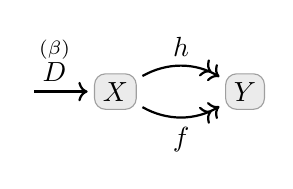
\begin{tikzpicture}[center base]
				\node[dpad0] (Y) {$Y$};
				\node[dpad0,left=1.1 of Y] (X) {$X$};
				%
				\draw[arr2, ->>] (X) to[bend left] node[pos=0.5, above]{$h$} (Y);
				\draw[arr2, ->>] (X) to[bend right] node[pos=0.5, below]{$f$} (Y);
				\draw[arr2, <-] (X) to node[pos=0.6, above]{$\overset{(\beta)}D$} +(-1.1, 0);
			\end{tikzpicture}}
		&=  \!\! \inf_{\substack{\mu(X)~\text{s.t.} \\ { \mathrm{supp}(\mu) \subseteq [f=h]}} } \beta \kldiv[\Big]{\mu(X)}{D(X)} \\
		&= \beta \kldiv[\Big]{ D \mid [f\!=\!h]}{ D } \\
		&= \beta \Ex_{D \mid f=h}
			\log \frac
				% {\mathbbm1[f\!=\!h](X)  D(X)}
				{\delta_{f=h}(X)  D(X)}
				{D(f\!=\!h)\cdot D(X)} \\
		&= \beta \Ex_{ D \mid f=h} \log \frac{1}{D(f\!=\!h)}
			& \hspace{-2em}{\color{gray}\left[ \begin{tabular}{c}
				% since $\mathbbm1[f\!=\!h](x) = 1$ for all $x$  that \\
				since $\delta_{f=h}(x) = 1$ for all $x$  that \\
				 contribute to the expectation \end{tabular} \right]} \\
		%&=	\inf_{\mu(X)} \Ex_{x \sim \mu} \beta \log \frac{\mu(x)}{D(x)} \\
		&= - \beta\, \log D(f=h)
			&  {\color{gray}\left[ \begin{tabular}{c}since $D(f=h)$ is a constant \end{tabular} \right]} \\
		&= - \beta\,\log \Big( \mathrm{accuracy}_{f,D} (h) \Big)\\
		&=  \beta\, \I_D[f=h].
	\end{align*}
\end{lproof}

\recall{prop:inc-two-gaussians}
\begin{lproof}\label{proof:inc-two-gaussians}
	Let $\dg M$ denote the PDG in question.
	%To simplify notation and emphasize their roles, we will write $\mu_1$ in place of $f(x)$, $\sigma_1$ in place of $t(x)$, and so forth.
	Since $D$ has high confidence, we know any joint distribution $\mu$ with a finite score must have $\mu(X) = D(X)$. Thus,
	\begin{align*}
		\aar{\dg M}_0 &= \inf_\mu \Ex_{x\sim D}\Ex_{y \sim\mu|x}
		 	\left[ \beta_1 \log \cfrac
				{\mu(y \mid x)}
				{\mathcal N(y \mid f(x), t(x))}
				%
				+  \beta_2 \log \cfrac
					{\mu(y \mid x)}
					{\mathcal N(y \mid h(x), s(x))}
				\right] \\
			&= \inf_\mu \Ex_{x\sim D}\Ex_{y \sim\mu|x}
			 	\left[ \beta_1 \log \frac
					{\mu(y \mid x)}
					{\frac{1}{t(x) \sqrt{2\pi}} \exp\left( -\frac{1}{2} \left(\frac{y-f(x)}{t(x)}\right)^2\right)}
					%
					+  \beta_2 \log \frac
						{\mu(y \mid x)}
						{\frac{1}{s(x) \sqrt{2\pi}} \exp\left( -\frac{1}{2} \left(\frac{y-h(x)}{s(x)}\right)^2\right)}
					\right] \\
			&= \inf_\mu \Ex_{x\sim D}\Ex_{y \sim\mu|x}
			 	\left[ \log \mu(y \mid x)^{\beta_1 + \beta_2}
					\begin{array}{l}
					+ \beta_1 \log( t(x) \sqrt{2\pi}) + \frac{\beta_1}{2} \left( \frac{y-f(x)}{t(x)} \right)^2\\
					+ \beta_2 \log( t(x) \sqrt{2\pi}) + \frac{\beta_2}{2} \left( \frac{y-h(x)}{s(x)} \right)^2
					\end{array}
					\right] \\
	\end{align*}

	{\centering\color{red}\tt\Large$\langle$ TODO: finish proof.  $\rangle$\par}
\end{lproof}

\recall{lemma:pdgdiv}
\begin{lproof}\label{proof:pdgdiv}
	\begin{align*}
	\aar[\bigg]{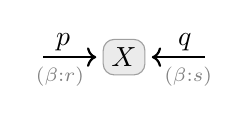
\begin{tikzpicture}[center base]
		\node[dpad0] (X) {$X$};
		\draw[arr2, <-] (X) --
				% node[above] {$\overset{(\beta : r)}p$}
				node[above, pos=0.6, inner sep=2pt, align=center] {$p$}
				node[below, pos=0.65, inner sep=3pt, align=center] {$\scriptstyle{\color{gray}(\beta : r)}$}
			++(-1.1,0);
		\draw[arr2, <-] (X) --
				% node[above,pos=0.5] {$\overset{(\beta : s)}q$}
				node[above, pos=0.6, inner sep=2pt, align=center] {$q$}
				node[below, pos=0.65, inner sep=3pt, align=center] {$\scriptstyle{\color{gray}(\beta : s)}$}
			 ++(1.1, 0);
	\end{tikzpicture}}
	&= \inf_\mu \Ex_\mu \log \frac{\mu(x)^{r+s}}{p(x)^r q(x)^s}\\
	&= (r+s) \inf_\mu \Ex_\mu  \left[ \log \frac{\mu(x)}{(p(x)^r q(x)^s)^{\frac1{r+s}}} \cdot \frac{Z}{Z} \right] \\
	&= \inf_\mu (r+s) \kldiv*{\mu}{\frac1Z p^{\frac r{r+s}} q^{\frac s{r+s}}} - (r+s) \log Z\\
	\intertext{where $Z := (\sum_x p(x)^r q(x)^s)^{\frac1{r+s}}$ is the constant required to normalize the denominator as a distribution. Since this is now a relative entropy, it achives its minimum when $\mu$ is the other distribution, at which point it contributes zero, so our formula becomes}
	&= - (r+s) \log Z \\
	&= - (r+s) \log  \sum_x \left(p(x)^{r}\vphantom{\Big|} q(x)^{s}\right)^{\frac{1}{r+s}}
	\quad\text{as promised.}
	\end{align*}
\end{lproof}


\recall{prop:regularized}
\begin{lproof}\label{proof:regularized}
\end{lproof}

\recall{prop:pdg-elbo-x}
\begin{lproof}\label{proof:pdg-elbo-x}
	Every distribution that does marginalize to $q(Z)$ or places any mass on $x' \ne x$ will have infinite score. Thus the only distribution that could have a finite score is $\mu(X,Z)$. Thus,

	\begin{align*}
	\aar[\Bigg]{
% 	  \Inc\left(
	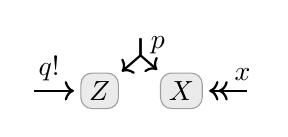
\begin{tikzpicture}[center base]
		\node[dpad0] (Z) {$Z$};
		\node[dpad0,right=.5 of Z] (X) {$X$};
		\coordinate (A) at ($ (X)!.5!(Z) + (0,0.7)$);
		\draw[arr1] (A) -- node[right]{$ p$} ++(0,-0.25) -- (X);
		\draw[arr1] (A) -- ++(0,-0.25) -- (Z);
%
		\draw[arr2, <<-] (X) --  node[above,pos=0.8]{$ x$} ++(0.9, 0);
		\draw[arr2, <-] (Z) -- node[above,pos=0.6]{$ q!$} ++(-0.9, 0);%
		% q^{\{\beta =\infty\}}
		% \ar[r,"p"] \& Z \ar[r,"p", bend left] \& X \ar[l,"q", bend left] \& \ar[l, two heads, "x"']
	\end{tikzpicture}
	}
	 &= \inf_\mu \bbr*{
% 	  \Inc\left(
		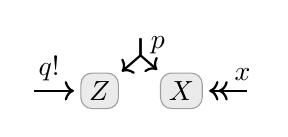
\begin{tikzpicture}[center base]
			\node[dpad0] (Z) {$Z$};
			\node[dpad0,right=.5 of Z] (X) {$X$};
			\coordinate (A) at ($ (X)!.5!(Z) + (0,0.7)$);
			\draw[arr1] (A) -- node[right]{$ p$} ++(0,-0.25) -- (X);
			\draw[arr1] (A) -- ++(0,-0.25) -- (Z);
%
			\draw[arr2, <<-] (X) --  node[above,pos=0.8]{$ x$} ++(0.9, 0);
			\draw[arr2, <-] (Z) -- node[above,pos=0.6]{$ q!$} ++(-0.9, 0);%
			% q^{\{\beta =\infty\}}
			% \ar[r,"p"] \& Z \ar[r,"p", bend left] \& X \ar[l,"q", bend left] \& \ar[l, two heads, "x"']
		\end{tikzpicture}
		}( \mu ) \\
	  &= \bbr*{
 % 	  \Inc\left(
 		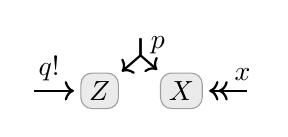
\begin{tikzpicture}[center base]
 			\node[dpad0] (Z) {$Z$};
 			\node[dpad0,right=.5 of Z] (X) {$X$};
 			\coordinate (A) at ($ (X)!.5!(Z) + (0,0.7)$);
 			\draw[arr1] (A) -- node[right]{$ p$} ++(0,-0.25) -- (X);
 			\draw[arr1] (A) -- ++(0,-0.25) -- (Z);
 %
 			\draw[arr2, <<-] (X) --  node[above,pos=0.8]{$ x$} ++(0.9, 0);
 			\draw[arr2, <-] (Z) -- node[above,pos=0.6]{$ q!$} ++(-0.9, 0);%
 			% q^{\{\beta =\infty\}}
 			% \ar[r,"p"] \& Z \ar[r,"p", bend left] \& X \ar[l,"q", bend left] \& \ar[l, two heads, "x"']
 		\end{tikzpicture}
 		}( \delta_x(X) q(Z) ) \\
	 &= \Ex_{\substack{x' \sim \delta_x \\ z \sim q}} \log \frac{\delta_x(x')q(z)} {p(x',z)}
	 = - \Ex_{z \sim q} \frac{p(x,z)}{q(z)} = - \mathrm{ELBO}_{p,q}(x).
	\end{align*}
\end{lproof}

We proove both \Cref{prop:pdg-elbo-vae} and \cref{prop:pdg-elbo-vae-whole} at the same time.
\recall{prop:pdg-elbo-vae}
% \recall{prop:pdg-elbo-vae-whole}
\begin{linked}{prop}{pdg-elbo-vae-whole}
	The following analog of \cref{prop:pdg-elbo-vae} for a whole dataset $\xsamp$ holds:
	\[
	-\Ex_{\datadist\xsamp}\mathrm{ELBO}_{p,e,d}(X) =
	 \aar*{
		% \begin{tikzcd}[AmpRep,row sep=1em,column sep=1.5em]
		% 	\ar[r,"p"] \& Z \ar[r,"d", bend left] \& X \ar[l,"e!", bend left] \& \ar[l, two heads, "x"']
		% \end{tikzcd}
		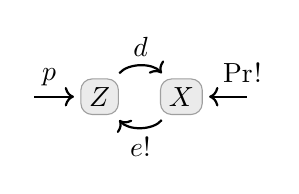
\begin{tikzpicture}[center base]
			\node[dpad0] (Z) {$Z$};
			\node[dpad0,right=.5 of Z] (X) {$X$};
			\draw[arr2, ->] (X) to[bend left=50]
				node[below]{$e!$} (Z);
			\draw[arr2, ->] (Z) to[bend left=50]
				node[above]{$d$} (X);
			\draw[arr2, <-] (X) --
				node[above,pos=0.8]{$\datadist\xsamp!$}
				++(0.9, 0);
			\draw[arr2, <-] (Z) --
				node[above,pos=0.6]{$p$}
				++(-0.9, 0);%
		\end{tikzpicture}} + \H(\datadist\xsamp). \]
\end{linked}
\begin{lproof}\label{proof:pdg-elbo-vae}\label{proof:pdg-elbo-vae-whole}
	The two proofs are similar. For \cref{prop:pdg-elbo-vae}, the optimal distribution must be $\delta_x(X) e(Z \mid X)$, and for \cref{prop:pdg-elbo-vae-whole}, it must be $\datadist\xsamp(X) e(Z \mid X)$, because $e$ and the data both have infinite confidence, so any other distribution gets an infinite score.
	At the same time, $d$ and $p$ define a joint distribution, so the inconsistency in question becomes
	\[
		\kldiv[\Big]{\delta_x(X) e(Z \mid X)}{p(Z)d(X\mid Z)}
			 = \Ex_{z \sim e \mid x} \left[ \log \frac{p(z)d(x\mid z)}{e(z \mid x)} \right] = \mathrm{ELBO}_{p,e,d}(x)
	\]
	in the first, case, and
	\begin{align*}
		\kldiv[\Big]{\datadist\xsamp(X) e(Z \mid X)}{p(Z)d(X\mid Z)}
		 &= \frac{1}{|\xsamp|}\sum_{x \in \xsamp} \Ex_{z \sim e \mid x} \left[ \log \frac{p(z)d(x\mid z)}{e(z \mid x)} + \log \frac{1}{\datadist\xsamp(x)} \right]\\
		 &= \mathrm{ELBO}_{p,e,d}(x) - \H(\datadist\xsamp)
	\end{align*}
	in the second.
\end{lproof}


Now, we formally state and prove the more general result for $\beta$-VaEs.

\begin{linked}{prop}{beta-elbo}
	The negative $\beta$-ELBO objective for a prior $p(X)$, encoder $e(Z \mid X)$, decoder $d(X \mid Z)$, at a sample $x$, is equal to the inconsistency of the corresponding PDG, where the prior has confidence equal to $\beta$. That is,
	\[
	-\beta\text{-}\mathrm{ELBO}_{p,e,d}(x) =
	 \aar**{
		% \begin{tikzcd}[AmpRep,row sep=1em,column sep=1.5em]
		% 	\ar[r,"p"] \& Z \ar[r,"d", bend left] \& X \ar[l,"e!", bend left] \& \ar[l, two heads, "x"']
		% \end{tikzcd}
		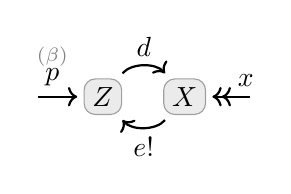
\begin{tikzpicture}[center base]
			\node[dpad0] (Z) {$Z$};
			\node[dpad0,right=.5 of Z] (X) {$X$};
			\draw[arr2, ->] (X) to[bend left=50]
				node[below]{$ e!$} (Z);
			\draw[arr2, ->] (Z) to[bend left=50]
				node[above]{$ d$} (X);
			\draw[arr2, <<-] (X) --
			  	node[above,pos=0.8]{$ x$}
			 	++(0.9, 0);
			\draw[arr2, <-] (Z) --
				node[above,pos=0.6]{$ \overset{{\color{gray}(\beta)}}p$}
				++(-0.9, 0);%
		\end{tikzpicture}}
	\]
\end{linked}
\begin{lproof} \label{proof:beta-elbo}
	\begin{align*}
		\aar*{\begin{tikzpicture}[center base]
			\node[dpad0] (Z) {$Z$};
			\node[dpad0,right=.5 of Z] (X) {$X$};
			\draw[arr2, ->] (X) to[bend left=50]
			   node[below]{$ e!$} (Z);
			\draw[arr2, ->] (Z) to[bend left=50]
			   node[above]{$ d$} (X);
			\draw[arr2, <<-] (X) --
			   node[above,pos=0.8]{$ x$}
			   ++(0.9, 0);
			\draw[arr2, <-] (Z) --
			   node[above,pos=0.6]{$\scriptstyle \overset{(\beta : \beta')}p$}
			   ++(-0.9, 0);%
	   \end{tikzpicture}}
	   	&= \inf_\mu \bbr[\Bigg]{\begin{tikzpicture}[center base]
 		   \node[dpad0] (Z) {$Z$};
 		   \node[dpad0,right=.5 of Z] (X) {$X$};
 		   \draw[arr2, ->] (X) to[bend left=50]
 			   node[below]{$ e!$} (Z);
 		   \draw[arr2, ->] (Z) to[bend left=50]
 			   node[above]{$ d$} (X);
 		   \draw[arr2, <<-] (X) --
 			   node[above,pos=0.8]{$ x$}
 			   ++(0.9, 0);
 		   \draw[arr2, <-] (Z) --
 			   node[above,pos=0.6]{$\scriptstyle \overset{(\beta : \beta')}p$}
 			   ++(-0.9, 0);%
 	   \end{tikzpicture}}(\mu) \\
	   &= \inf_\mu \Ex_{\mu(X,Z)} \left[ \beta \log \frac{\mu(Z)}{p(Z)} + \log \frac{\mu(X,  Z)}{\mu(Z) d(X \mid Z)} \right] \\
   \intertext{As before, the only candidate for a joint distribution with finite score is $\delta_x(X) e(Z \mid X)$. Note that the marginal on $Z$ for this distribution is itself, since $\int_x \delta_x(X) e(Z \mid X)\;\mathrm dx = e(Z \mid x)$. Thus, our equation becomes}
	   &= \Ex_{\delta_x(X) e(Z \mid X)} \left[ \beta \log \frac{e(Z \mid x)}{p(z)} + \log \frac{\delta_x(X) e(Z \mid X)}{e(Z \mid x) d(x \mid Z)} \right] \\
	   &= \Ex_{e(Z \mid x)} \left[ \beta \log \frac{e(Z \mid x)}{p(Z)} + \log \frac{1}{ d(x \mid Z)} \right]
	   \qquad = -\beta\text{-}\mathrm{ELBO}_{p,e,d}(x).
	\end{align*}
\end{lproof}


\recall{prop:fg-inconsistency-is-partition-function}
\begin{lproof}\label{proof:fg-inconsistency-is-partition-function}
	\def\theelt{\mathop{\mathrm{the}}}
	Let $\theelt(\{x\}) := x$ be a function that extracts the unique element singleton set.
	We showed in the orignal paper (Corolary 4.4.1) that
	\[ \theelt \bbr{(\UPDGof{\Phi}, \theta, \theta)}^*_1 = \Pr\nolimits_{\Phi, \theta}(\mat w)
		= \frac{1}{Z_\Psi} \prod_{j} \phi_j(\mat w_j)^{\theta_j}. \]
	Recall the statement of Prop 4.6 from the original paper,
	\begin{equation}\label{eqn:nice-score-repeated}
		\bbr{\dg M}_\gamma(\mu) = \Ex_{\mat w \sim \mu}\! \Bigg\{ \sum_{ X \xrightarrow{\!\!L} Y  } \bigg[\,
		   \!\beta_L \log \frac{1}{\bp(y^{\mat w} |x^{\mat w})} +
		   {\color{red}(\gamma\alpha_L - \beta_L ) \log \frac{1}{\mu(y^{\mat w} |x^{\mat w})}} \bigg] -
		\gamma \log \frac{1}{\mu(\mat w)}  \Bigg\}, \\
	\end{equation}
	but note that since $\gamma = 1$, and $\alpha,\beta$ are both equal to $\theta$ for our PDG
	 (since $\PDGof{\Psi} = \PDGof{(\Phi,\theta)} = (\UPDGof\Phi, \theta,\theta)$), the middle term disappears, yielding the standard variational free energy $\VFE(\mu)$.
	Recall also that
	$\aar{\dg M}_\gamma = \inf_\mu \bbr{\dg M}_\gamma(\mu)$ and $\bbr{\dg M}^*_\gamma = \arg\min \bbr{\dg M}_\gamma(\mu)$, so (with a minor abuse of notation), $\aar{\dg M}_\gamma = \bbr{\dg M}_\gamma(\bbr{\dg M}_\gamma^*)$. We now compute the value of the inconsistency $\aar{(\UPDGof\Phi, \theta,\theta)}_1$.
	\begin{align*}
		\aar{(\UPDGof{\Phi}, \theta, \theta)}_1
		&= \bbr{(\UPDGof{\Phi}, \theta, \theta)}_1\Big(\Pr\nolimits_{\Phi, \theta}(\mat w) \Big) \\
		%\frac{1}{Z_\Phi} \prod_j \phi_j(\mat w_j)^{\theta_j}
		&=
		 \Ex_{\mat w \sim \mu}\! \Bigg\{ \sum_{X \xrightarrow{\!\!L} Y} \bigg[\,
	      		\!\beta_L \log \frac{1}{\bp(y^{\mat w} |x^{\mat w})}
				% (\alpha_L - \beta_L ) \log \frac{1}{\mu(y^{\mat w} |x^{\mat w})}
				\bigg] - \log \frac{1}{\Pr\nolimits_{\Phi, \theta}(\mat w) }  \Bigg\}
			& \Big[	 ~\text{by \eqref{eqn:nice-score-repeated}}~	\Big]\\
		&=
		 \Ex_{\mat w \sim \mu}\! \Bigg\{ \sum_j \bigg[\,
	      		\!\theta_j \log \frac{1}{\phi_j(\mat w_j)}
				\bigg] - \log \frac{Z_\Psi}{\prod_{j} \phi_j(\mat w_j)^{\theta_j}}  \Bigg\}
			& \Big[ \parbox{1.5in}{\centering%
			 	cpds $\bp$ correspond\\ to factors $\phi_j$}	\Big]\\
		&=
		 \Ex_{\mat w \sim \mu}\! \Bigg\{ \sum_j \bigg[\,
	      		\!\theta_j \log \frac{1}{\phi_j(\mat w_j)}
				\bigg] - \sum_j \left[\theta_j \log \frac{1}{\phi_j(\mat w_j)} \right]
				 - \log Z_\Psi \Bigg\} \\
		&= \Ex_{\mat w \sim \mu} [- \log Z_\Psi] \\
		&= - \log Z_\Psi & \Big[~\text{$Z_\Psi$ is constant in $\mat w$}~\Big]
	\end{align*}
\end{lproof}

\section{More Notes}
\subsection{Surprise}
A common justification for using $\I_p(x)$ as a cost for updating a probabilistic model $p(x)$ based on an observed sample $x$, is that by minimizing it, you  ``maximize the probability of seeing your data''.%
%
 	\footnote{this justification should not be taken too seriously  without constraints on $p$, because the optimal value of $p$  is $\delta_x$, which does not generalize.}
But this explanation applies just as well to $-p(x)$. Why include the logarithm?
There are plenty of answers to this question; among them: $\I_p$ is convex in $p$, it decomposes products into arguably simpler sums, is more numerically stable, has a well-defended physical analogue in thermodynamics, and is a primative of information theory.

For those after a quick and rigorous justification (as opposed to handwaving or a thermodynamics textbook), none of these answers are entirely satisfying.
They suggest that $\I_p$ has certain nice properties, but not that it enjoys them uniquely, or that no other loss function satisfies nicer ones.
Pedagogically speaking, the situation is more straightforward for us.
Although PDG semantics themselves require non-trivial justification%
 	% (e.g., by direct appeal to information theory)
, they give us in return uniform answers to many questions, starting with:
Why use the surprise $\I_p(x)$, to measure the loss of a model $p(X)$ on sample $x$? Because it is the inconsistency of simultanously believing $X = x$ and $X \sim p$.


\end{document}
